\documentclass{beamer}
\usepackage{amsfonts}
\usepackage{siunitx}
\usepackage{booktabs}
\usepackage{xcolor}
\usepackage{mathtools}
\usepackage{amsthm}
\usepackage{natbib}
\usepackage{bbm}
\usepackage{centernot}

\title{A Rigorous Framework for Automated Design Assessment and Type I Error Control}

% I honestly don't really care about the order,
% but from an audience perspective, the one who's presenting may want to put their name first?
% Currently, it is set to the same ordering as in the paper.
\author[shortname]{James Yang\inst{1,2} \and T. Ben Thompson\inst{2} \and Michael Sklar\inst{2}} 
\institute[shortinst]{\inst{1} Stanford University \and
                      \inst{2} Confirm Solutions}
\date{\today}

\newcommand{\prob}{\mathbb{P}}
\newcommand{\pr}[1]{\left( #1 \right)}
\newcommand{\br}[1]{\left[#1\right]}
\newcommand{\sbr}[1]{\left\{#1\right\}}
\newcommand{\normal}{\mathcal{N}}
\newcommand{\set}[1]{\{#1\}}
\newcommand{\EEE}{\mathbb{E}}
\newcommand{\R}{\mathbb{R}}
\newcommand{\design}{\mathcal{D}}
\newcommand{\indic}[1]{\mathbbm{1}_{#1}}
\newcommand{\norm}[1]{\left\|#1\right\|}
\DeclareMathOperator{\var}{Var}
\DeclareMathOperator{\expit}{expit}
\DeclareMathOperator{\logit}{logit}
\DeclareMathOperator{\Binom}{Binom}
\DeclarePairedDelimiter\floor{\lfloor}{\rfloor}

\beamertemplatenavigationsymbolsempty
\begin{document}

\frame{\titlepage}

\begin{frame}
\frametitle{Table of Contents}
\tableofcontents
\end{frame}

\section{Introduction}%
\frame{\tableofcontents[currentsection]}

\begin{frame}{Pharma R\&D is Growing}
\begin{figure}
    \centering
    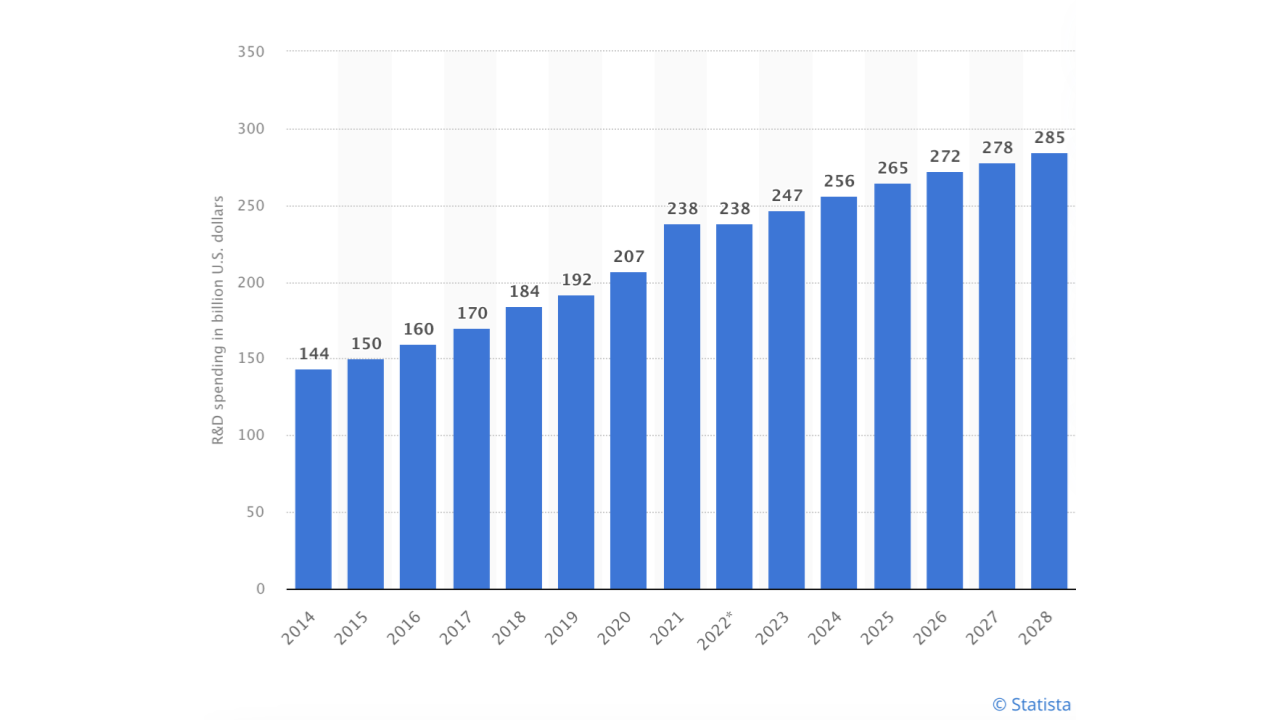
\includegraphics[width=\linewidth]{figs/pharma_growing.png}
\end{figure}
\end{frame}

\begin{frame}{Eroom's Law: Efficiency Down}
\begin{figure}
    \centering
    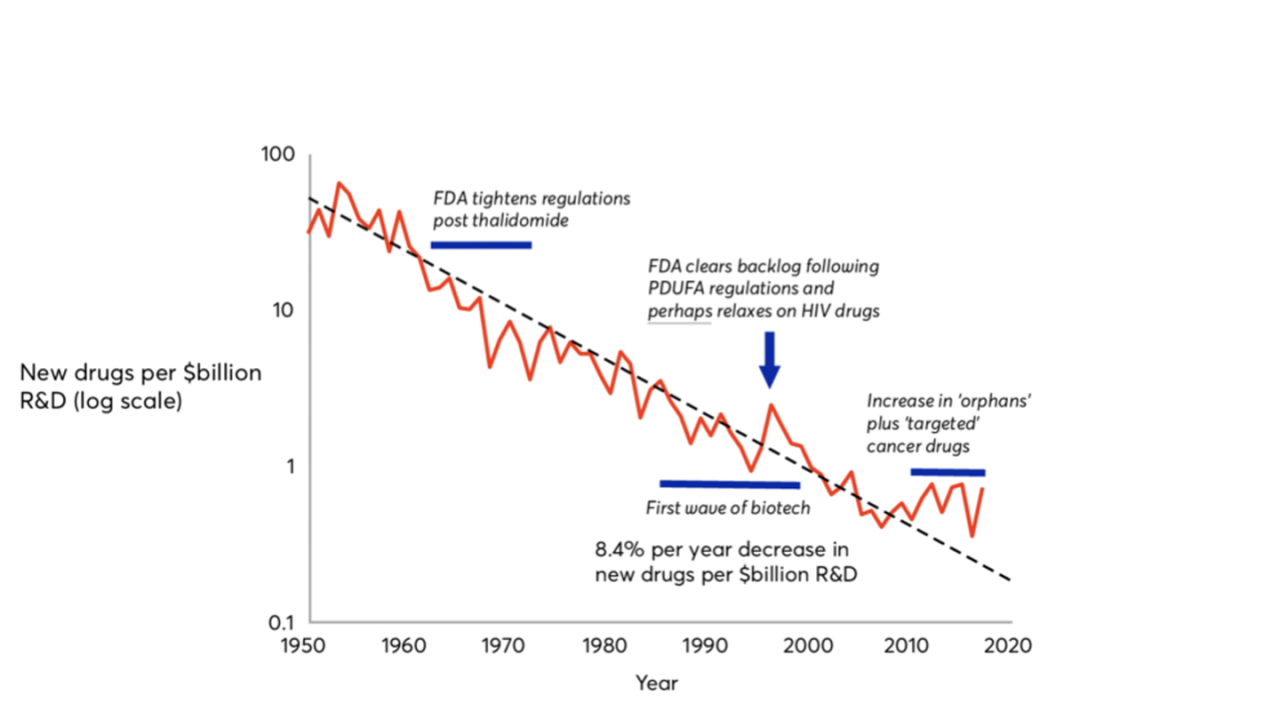
\includegraphics[width=\linewidth]{figs/efficiency_down.png}
\end{figure}    
\end{frame}

\begin{frame}{Covid Put a Focus on Shortening Clinical Trials}
\begin{figure}
    \centering
    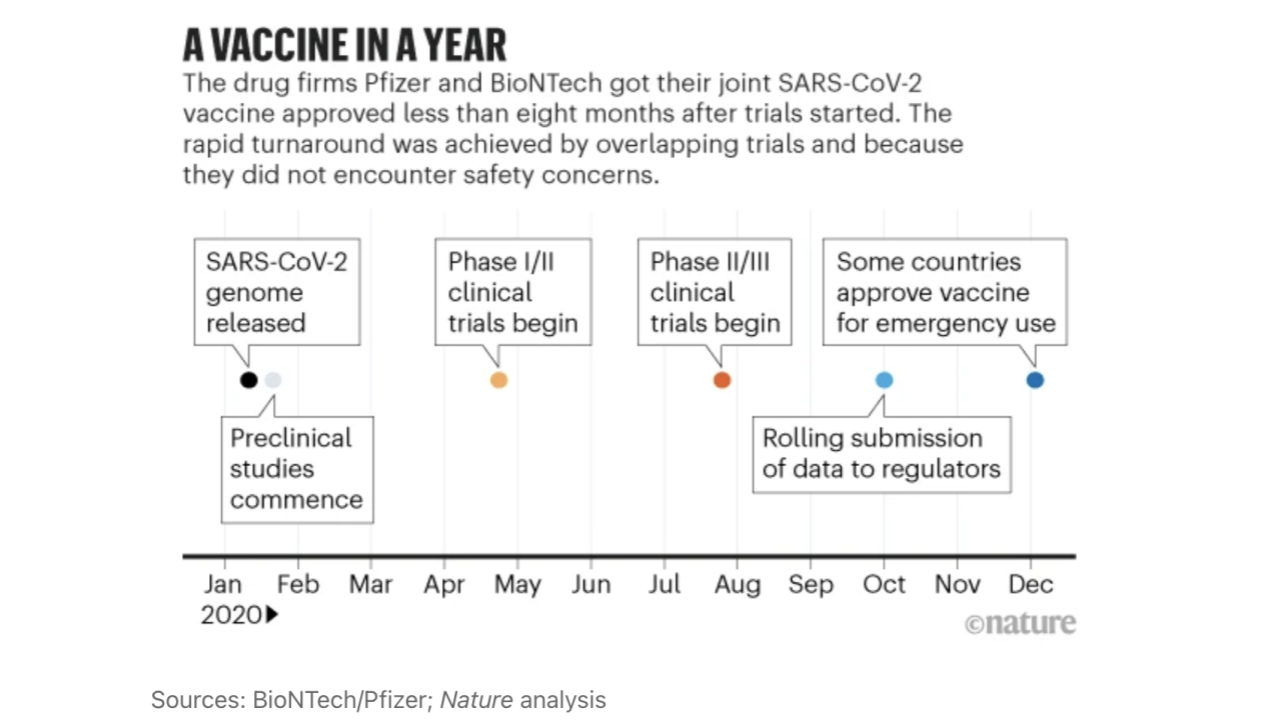
\includegraphics[width=\linewidth]{figs/covid.png}
\end{figure}    
\uncover<2->{
\textbf{How can statisticians speed up the clinical trials system?}
}
\end{frame}

\begin{frame}{Add Features to Improve Trial Efficiency}
\begin{itemize}
    \item Smoothly combine studies (e.g. Phase I/II, or II/III).
    \item Stop early for success (efficacy), or failure (futility).
    \item Compare multiple treatments or doses to select the best.
    \item Adaptive sample sizing.
    \item Use of outside data.
\end{itemize} 
\end{frame}

\begin{frame}{Problem: Analytic Control goes Out the Window!}
\textbf{Adaptive T-Test:}
\begin{itemize}
    \item $X_i \sim \normal(\mu, \sigma^2)$ (unknown $\mu, \sigma$).
    \item $H_0: \mu = 0$.
    \item Total of $6$ analyses.
    \item Before each analysis, add $10$ i.i.d. samples.
    \item At each analysis $i$, reject if 
    \begin{align*}
        T_i := \frac{\sqrt{N_i} \bar{X}_i}{\hat{\sigma}_i} > 2
        \quad \text{and} \quad
        \bar{X}_i > 0.1
    \end{align*}
\end{itemize}
\uncover<2->{%
\begin{center}
\textbf{What is the Type I Error?}
\end{center}
}
\uncover<3->{%
\begin{center}
Classical toolkit breaks even with Gaussian data.
\end{center}
}
\end{frame}

\begin{frame}{Adaptive T-Test Non-Trivial Null Distribution}
\begin{figure}
    \centering
    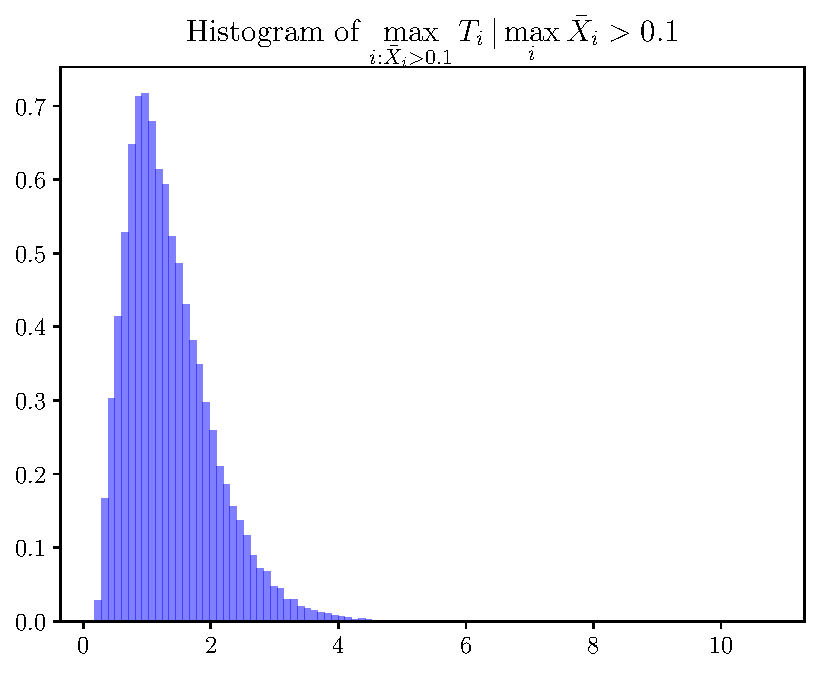
\includegraphics[width=0.8\linewidth]{figs/introduction_att_hist.pdf}
    \caption{Adaptive T-Test test statistic distribution for $\sigma \equiv 1$.}
\end{figure}
\end{frame}

\begin{frame}{Intermediate Techniques Fail}
\begin{itemize}
    \item Composite null with nuisance parameters (noise levels).
    \begin{center}
        \textbf{Simulating on single null point $\centernot\implies$ Type I Error control.}
    \end{center}
    \item Sharp null hypothesis (exact zero causal effect) is usually false (“null” treatments often increase the variability of outcomes).
    \begin{center}
        \textbf{Breaks permutation methods.}
    \end{center}
    \item Adaptive sampling renders the test statistic to be non-pivotal.
    \begin{center}
        \textbf{Breaks the bootstrap.}
    \end{center}
\end{itemize} 
\end{frame}

\begin{frame}{Simulation to the Rescue?}
\begin{figure}
    \centering
    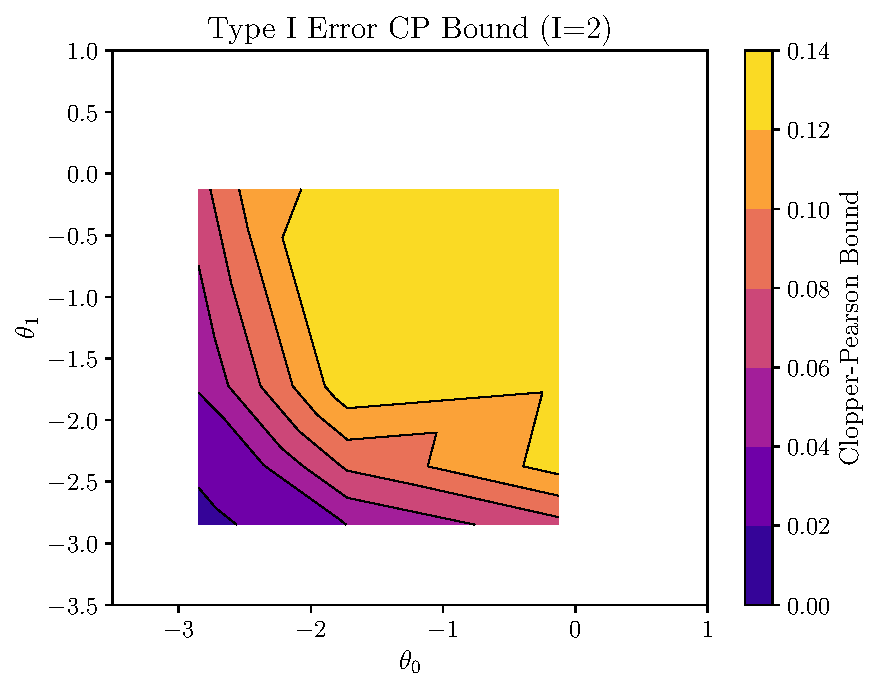
\includegraphics[width=0.9\linewidth]{figs/introduction_rescue_0.pdf}
\end{figure}
\begin{center}
    \textbf{To accept or not to accept?}
\end{center}
\end{frame}

\begin{frame}{Simulation to the Rescue?}
\begin{figure}
    \centering
    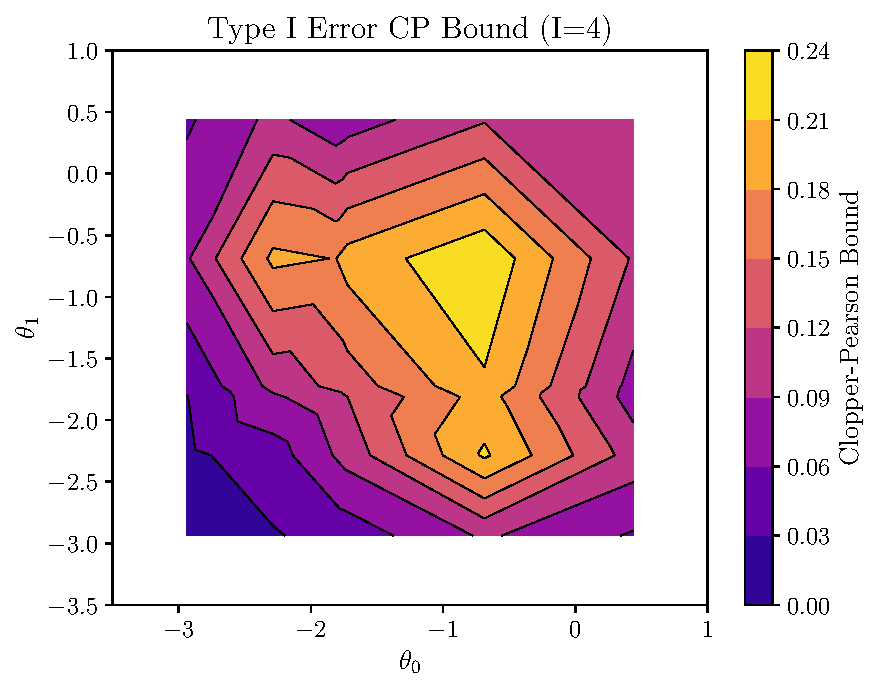
\includegraphics[width=0.9\linewidth]{figs/introduction_rescue_1.pdf}
\end{figure}
\begin{center}
    \textbf{To accept or not to accept?}
\end{center}
\end{frame}

\begin{frame}{Simulation to the Rescue?}
\begin{figure}
    \centering
    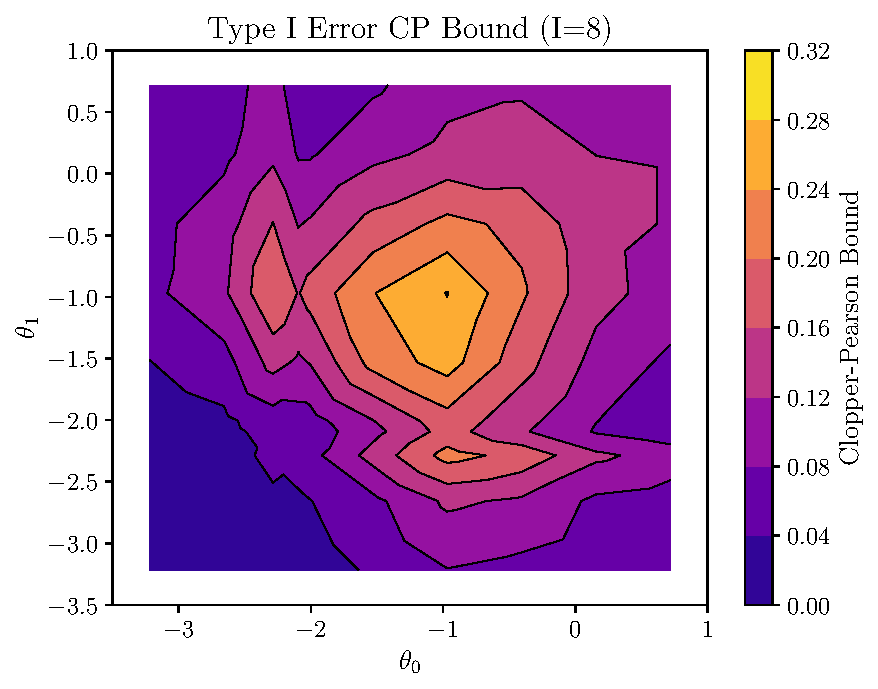
\includegraphics[width=0.9\linewidth]{figs/introduction_rescue_2.pdf}
\end{figure}
\begin{center}
    \textbf{To accept or not to accept?}
\end{center}
\end{frame}

\begin{frame}{Simulation to the Rescue?}
\begin{figure}
    \centering
    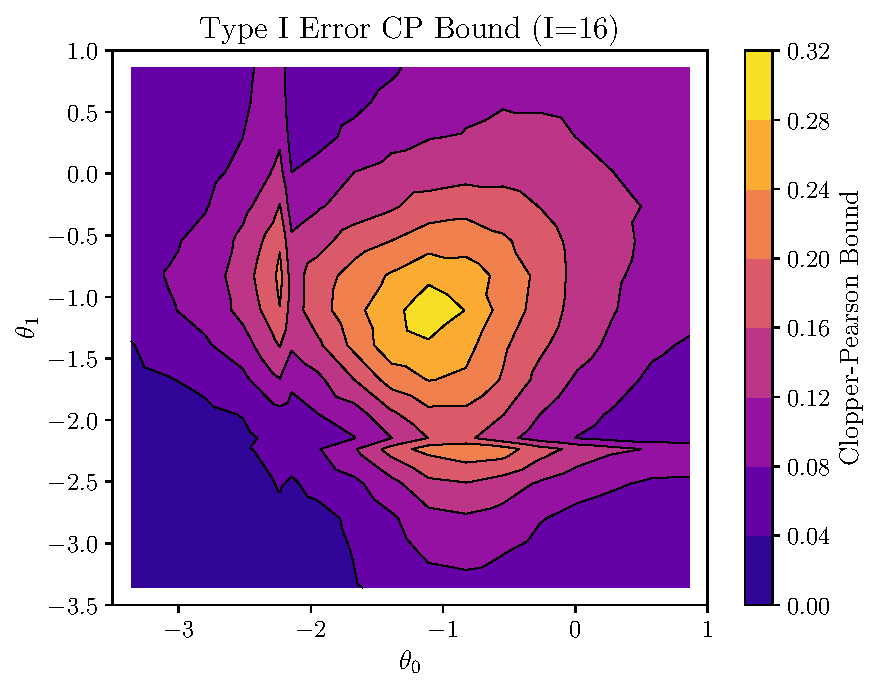
\includegraphics[width=0.9\linewidth]{figs/introduction_rescue_3.pdf}
\end{figure}
\begin{center}
    \textbf{To accept or not to accept?}
\end{center}
\end{frame}

\begin{frame}{Simulation to the Rescue?}
\begin{figure}
    \centering
    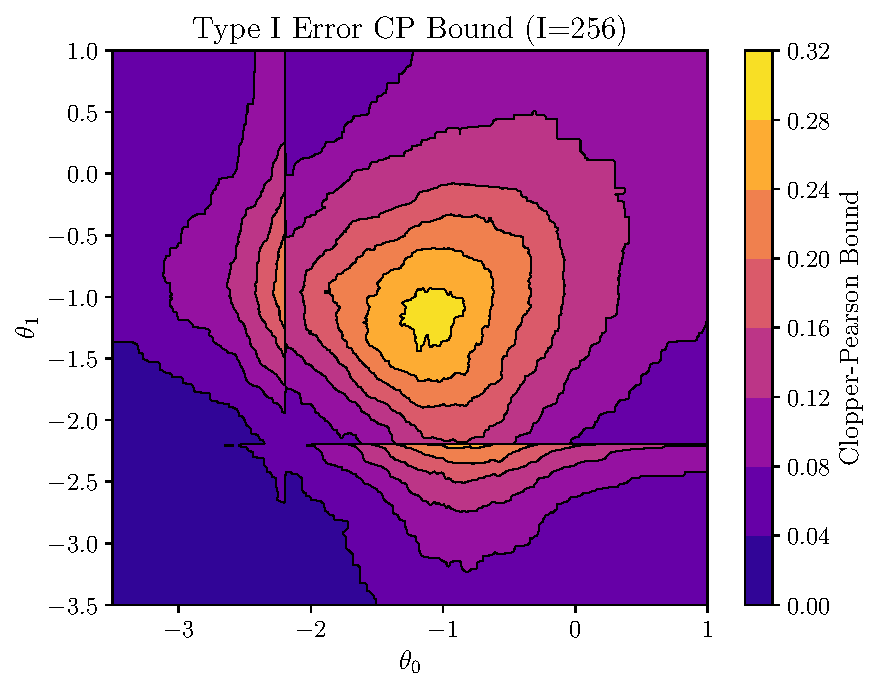
\includegraphics[width=0.9\linewidth]{figs/introduction_rescue_4.pdf}
\end{figure}
\begin{center}
    \textbf{To accept or not to accept?}
\end{center}
\end{frame}

\begin{frame}{Simulation Raises New Challenges}
\begin{itemize}
    \item Simulation constrained to \textbf{finite} number of null points.
    \begin{center}
        \textbf{How do we deal with composite nulls?}
    \end{center}
    \item Simulation has Monte Carlo error. 
    \begin{center}
        \textbf{How do we deal with Monte Carlo error?}
    \end{center}
    \item Bounded computing power.
    \begin{center}
        \textbf{How many points in the null space to simulate?}
    \end{center}
    \begin{center}
        \textbf{Are the simulations even tractable?}
    \end{center}
\end{itemize}
\end{frame}

\begin{frame}{Intuition of Our Approach}
\begin{figure}
    \centering
    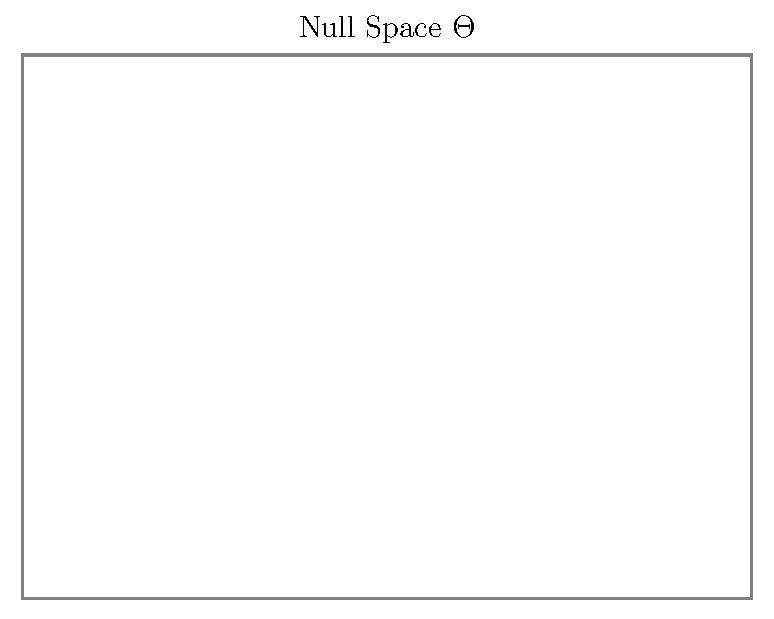
\includegraphics[width=0.95\linewidth]{figs/approach_1.pdf}
\end{figure} 
\end{frame}

\begin{frame}{Partition $\Theta$ into Tiles with Representatives}
\begin{figure}
    \centering
    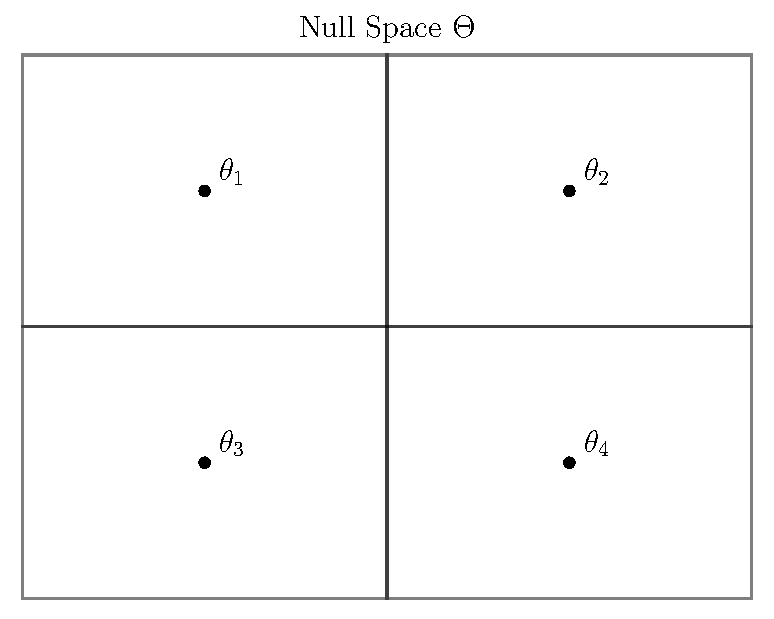
\includegraphics[width=0.95\linewidth]{figs/approach_2.pdf}
\end{figure} 
\end{frame}

\begin{frame}{Simulate on each Representative}
\begin{figure}
    \centering
    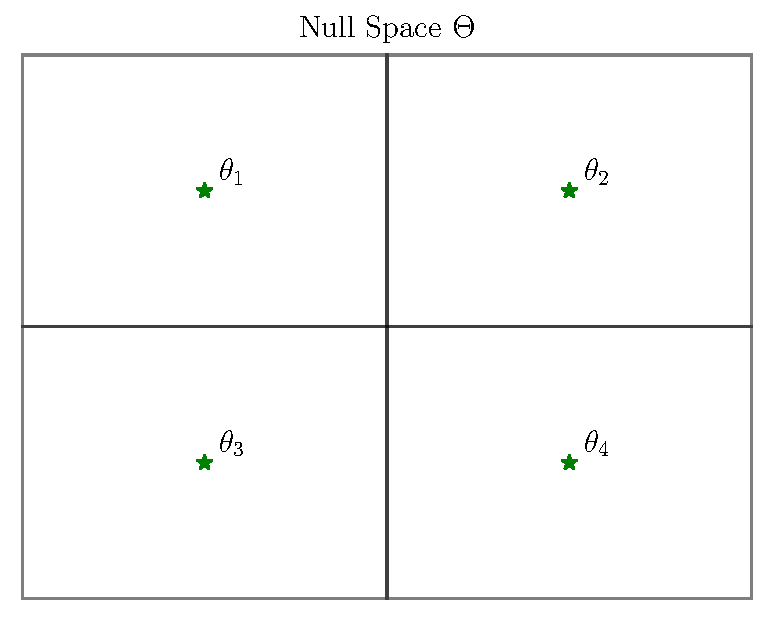
\includegraphics[width=0.95\linewidth]{figs/approach_3.pdf}
\end{figure} 
\end{frame}

\begin{frame}{Extend Simulation Information to Tile}
\begin{figure}
    \centering
    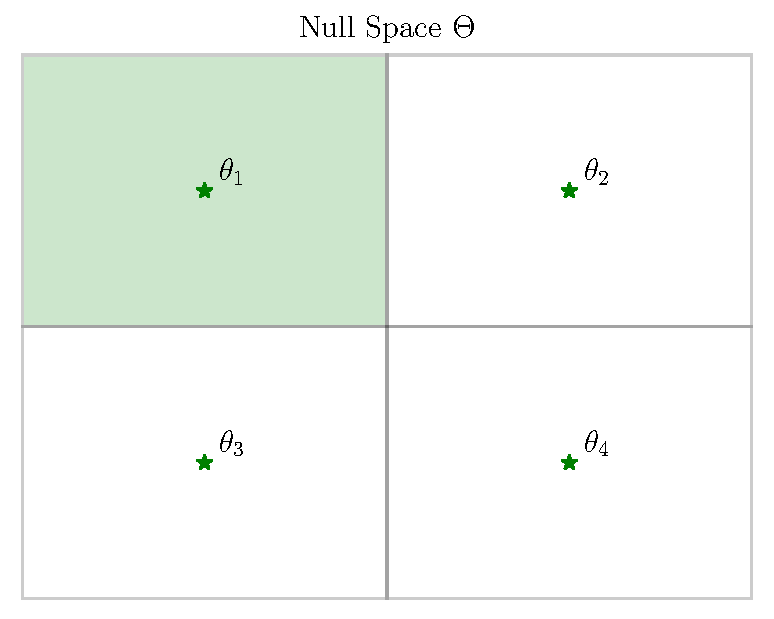
\includegraphics[width=0.95\linewidth]{figs/approach_4.pdf}
\end{figure} 
\end{frame}

\begin{frame}{Divide-and-Conquer for Guarantees on All of $\Theta$}
\begin{figure}
    \centering
    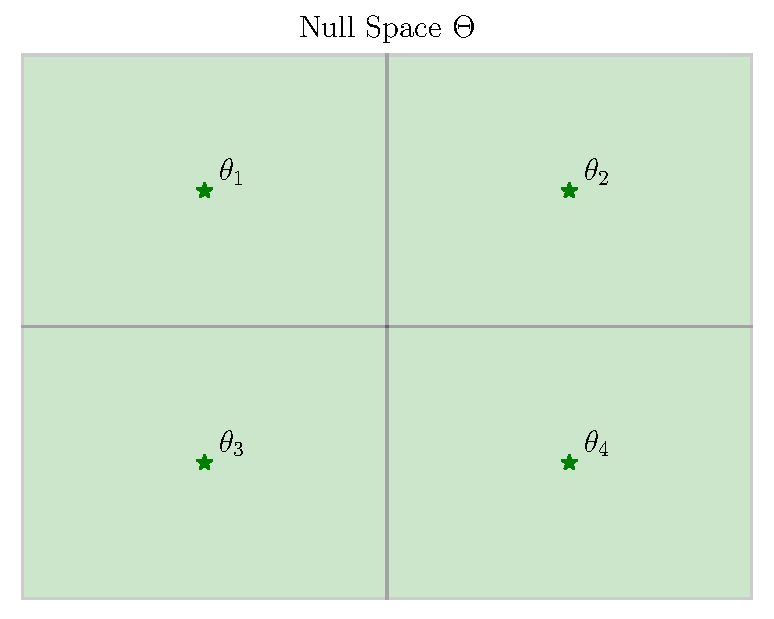
\includegraphics[width=0.95\linewidth]{figs/approach_5.pdf}
\end{figure} 
\end{frame}

\begin{frame}{Our Approach: Proof-by-Simulation}
\textbf{General Workflow:}
\begin{itemize}
    \item Let $\Theta$ be a (bounded) null hypothesis space.
    \item Partition $\Theta$ into tiles $\set{\Theta_i}_{i=1}^I$ 
        with representatives $\set{\theta_i}_{i=1}^I$.
    \item Simulate the design on each $\theta_i$ and output test statistics.
    \item Use our method \textbf{Continuous Simulation Extension} (CSE) to 
        \emph{extend} information at each $\theta_i$ to any other point in $\Theta_i$.
    \item Divide-and-conquer to get guarantees on \emph{all of $\Theta$}.
\end{itemize}
\end{frame}

\begin{frame}{Method 1: Validation for Point-wise Confidence}
\begin{figure}
    \centering
    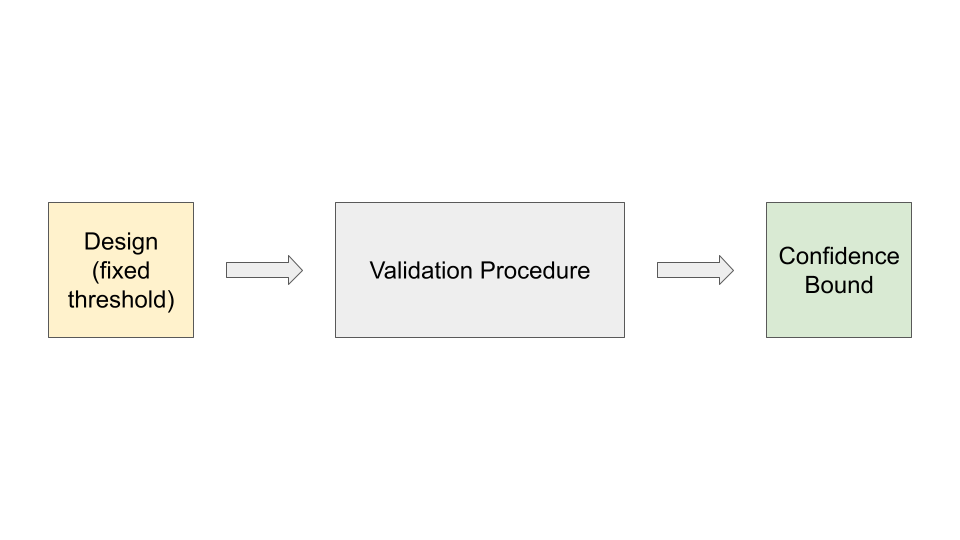
\includegraphics[width=\linewidth]{figs/validation_scheme.png}
\end{figure}
\end{frame}

\begin{frame}{Method 1: Validation for Point-wise Confidence}
\begin{itemize}
    \item \textbf{Validation}: 
        Construct bounds $(\hat{l}(\cdot), \hat{u}(\cdot))$
        for the true Type I Error, $f(\cdot)$, with confidence $1-\delta$:
        \begin{align*}
            \forall \theta \in \Theta ,\, 
            &\prob\pr{\hat{l}(\theta) \leq f(\theta)} \geq 1-\delta \text{ and } \\
            &\prob\pr{\hat{u}(\theta) \geq f(\theta)} \geq 1-\delta
        \end{align*}
    \item Point-wise guarantee is appropriate since 
        there is only one \emph{true} value of $\theta$.
\end{itemize} 
\end{frame}

\begin{frame}{Method 2: Calibration for Type I Error Proof}
\begin{figure}
    \centering
    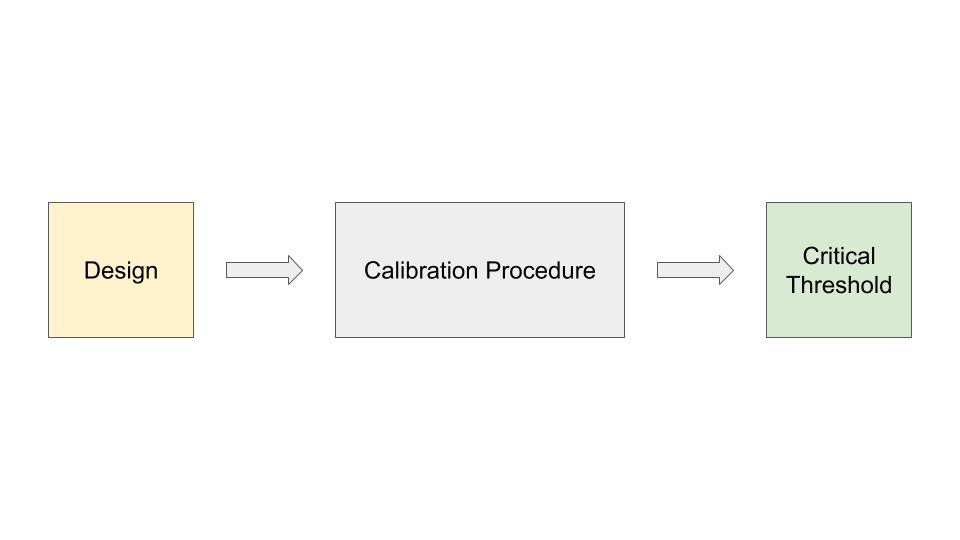
\includegraphics[width=\linewidth]{figs/calibration_scheme.png}
\end{figure}
\end{frame}

\begin{frame}{Method 2: Calibration for Type I Error Proof}
\begin{itemize}
    \item \textbf{Calibration}: 
        Select a (random) critical threshold, $\hat{\lambda}^*$, such that 
        \begin{align*}
        \forall \theta \in \Theta,\, 
        \EEE\br{f_{\hat{\lambda}^*}(\theta)} 
        \leq 
        \alpha
        \end{align*}
        where $f_{\lambda}(\theta)$ is the Type I Error at $\theta$
        using threshold $\lambda$.
\end{itemize} 
\end{frame}

\begin{frame}{Random $\hat{\lambda}^*$ is acceptable}
\begin{itemize}
    \item Guarantee is \textbf{overall} valid (regulators want this!).
    \item Practitioners \textbf{already use} simulations to evaluate designs.
    \item Our approach is \textbf{strictly stronger} because we can give guarantees.
\end{itemize}
\end{frame}
\section{Methodology}

\subsection{Continuous Simulation Extension (CSE): Tilt-Bound}
\frame{\tableofcontents[currentsubsection]}

\begin{frame}{Main Task: Find Type I Error at $\theta$}
\begin{figure}
    \centering
    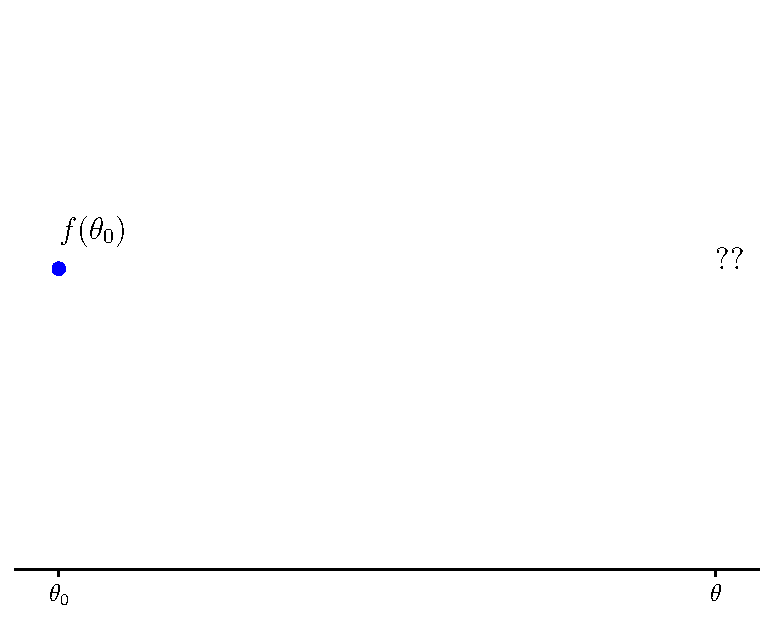
\includegraphics[width=0.75\linewidth]{figs/cse_problem.pdf}
\end{figure}
\begin{itemize}
    \item $X \sim P_\theta$ (known distribution), null space $\Theta$.
    \item Any arbitrary design $\design$.
    \item $f(\theta) := \prob_\theta\pr{\design \text{ rejects}}$.
\end{itemize} 
\end{frame}

\begin{frame}{Main Task: Find \textbf{Upper Bound} of Type I Error at $\theta$}
\begin{figure}
    \centering
    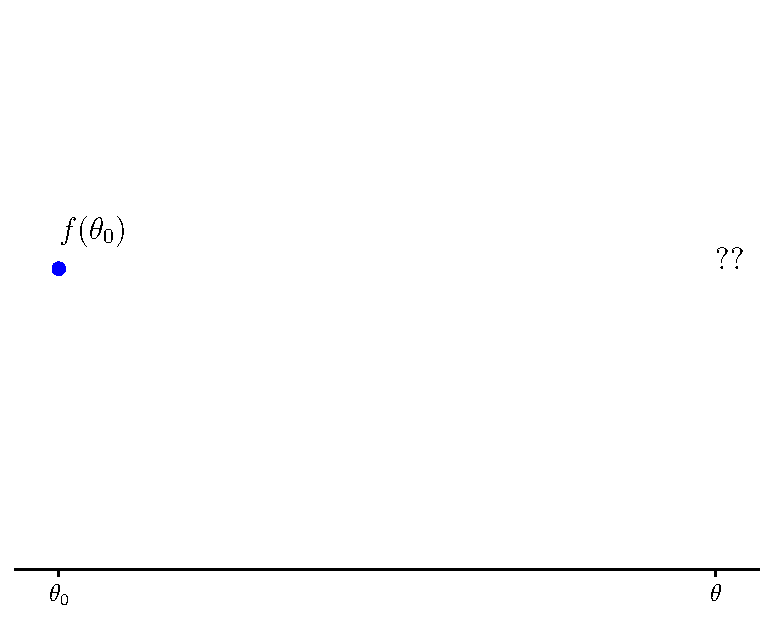
\includegraphics[width=0.75\linewidth]{figs/cse_problem.pdf}
\end{figure}
\begin{itemize}
    \item $X \sim P_\theta$ (known distribution), null space $\Theta$.
    \item Any arbitrary design $\design$.
    \item $f(\theta) := \prob_\theta\pr{\design \text{ rejects}}$.
\end{itemize} 
\end{frame}

\begin{frame}{Main Task: Find \textbf{Upper Bound} of Type I Error at $\theta$}
\begin{figure}
    \centering
    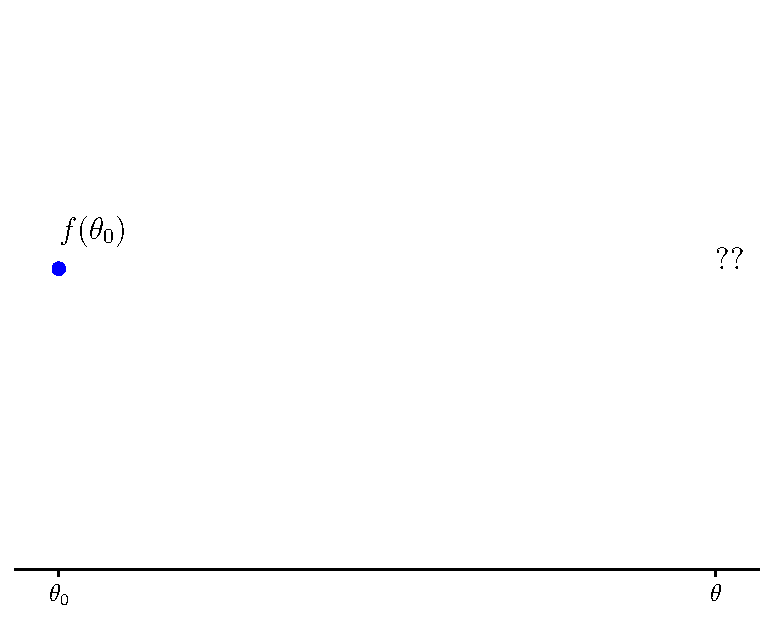
\includegraphics[width=0.75\linewidth]{figs/cse_problem.pdf}
\end{figure}
\begin{itemize}
    \item Assume further that $P_\theta$ is an \textbf{exponential family}.
    \item Does this help?
\end{itemize}
\end{frame}

\begin{frame}{Main Task: Find \textbf{Upper Bound} of Type I Error at $\theta$}
\begin{figure}
    \centering
    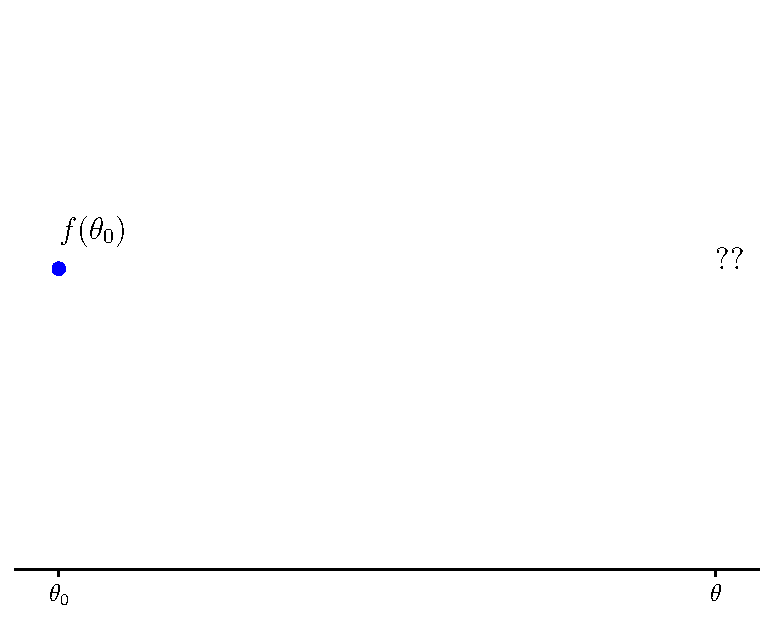
\includegraphics[width=0.75\linewidth]{figs/cse_problem.pdf}
\end{figure}
\begin{itemize}
    \item Assume further that $P_\theta$ is \textbf{Gaussian}.
    \item Does this help?
\end{itemize}
\end{frame}

\begin{frame}{Intuition for Upper Bounding the Type I Error}
\begin{itemize}
    \item \textbf{Morally}, distribution assumptions \emph{should} help!
    \item Use \textbf{``curvature''} information in distribution.
    \item \textbf{Restrict} the possible values for $f(\theta)$.
\end{itemize} 
\end{frame}

\begin{frame}{Claim: Upper Bound on the Type I Error}
\begin{figure}
    \centering
    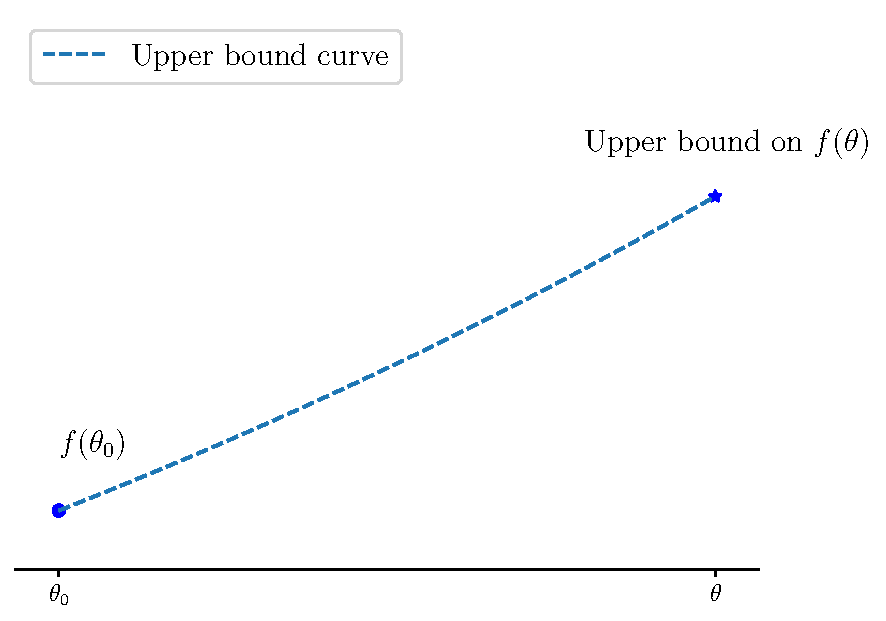
\includegraphics[width=\linewidth]{figs/cse_solution.pdf}
\end{figure} 
\end{frame}

\begin{frame}{Derivation: Begin with a Change of Measure}
Let $A := \set{x : \design(x) \text{ rejects}}$.

Then,
\begin{align*}
    f(\theta)
    &=
    \EEE_\theta\br{\indic{X \in A}}
    =
    \EEE_{\theta_0}\br{\indic{X \in A} \frac{p_\theta(X)}{p_{\theta_0}(X)}}
\end{align*}
\end{frame}

\begin{frame}{Use H\"{o}lder's Inequality!}
For any $p, q \geq 1$ such that $\frac{1}{p} + \frac{1}{q} = 1$,
\begin{align*}
    f(\theta) 
    &\leq
    \norm{\indic{X \in A}}_{L^p(P_{\theta_0})}
    \norm{\frac{p_\theta(X)}{p_{\theta_0}(X)}}_{L^q(P_{\theta_0})}
    \\&=
    f(\theta_0)^{1-\frac{1}{q}} 
    \norm{\frac{p_\theta(X)}{p_{\theta_0}(X)}}_{L^q(P_{\theta_0})}
\end{align*} 
\end{frame}

\begin{frame}{Introduce Distributional Assumptions}

Let $P_\theta$ have a density of the form:
\begin{align*}
    p_\theta(x)
    =
    \exp\sbr{g_\theta(x) - A(\theta)}
\end{align*}

By a simple calculation, one can show that
\begin{equation*}
    \norm{\frac{p_\theta(X)}{p_{\theta_0}(X)}}_{L^q(P_{\theta_0})}
    =
    \exp\sbr{
        \frac{\psi(\theta_0, \theta-\theta_0, q)}{q}
        - \psi(\theta_0, \theta-\theta_0, 1)
    }
\end{equation*} 
\begin{equation*}
    \psi(\theta_0, v, q)
    :=
    \log\EEE_{\theta_0}\br{\exp\sbr{q\pr{g_{\theta_0+v}(X)-g_{\theta_0}(X)}}}
\end{equation*} 
\end{frame}

\begin{frame}{We did it!}
For any $q \geq 1$,
\begin{align*}
    f(\theta)
    &\leq
    f(\theta_0)^{1 - \frac{1}{q}}
    \exp\sbr{\frac{\psi(\theta_0, \theta-\theta_0, q)}{q} - \psi(\theta_0, \theta-\theta_0, 1)}
\end{align*}
\end{frame}

\begin{frame}{Tilt-Bound and Special Cases}
\textbf{Tilt-Bound ($q \geq 1$):}
\begin{equation*}
    U(\theta_0, v, q, f(\theta_0))
    :=
    \underbrace{f(\theta_0)^{1 - \frac{1}{q}}}_{
    \mathclap{\textcolor{red}{\theta_0 \textbf{ info}}}
    }
    \underbrace{\exp\sbr{\frac{\psi(\theta_0, v, q)}{q} - \psi(\theta_0, v, 1)}}_{
    \mathclap{\textcolor{red}{\textbf{Curvature info}}}
    }
\end{equation*}
\textbf{Exponential family:}
\begin{equation*}
    \psi(\theta_0, v, q) 
    :=
    A(\theta_0 + qv) - A(\theta_0)
\end{equation*}
\textbf{Normal family $\set{\normal\pr{\theta, 1} : \theta \in \Theta}$:}
\begin{equation*}
    U(\theta_0, v, q, f(\theta_0))
    :=
    f(\theta_0)^{1 - \frac{1}{q}} 
    \exp\sbr{\frac{(q - 1) v^2}{2}}
\end{equation*}
\end{frame}

\begin{frame}{Optimize over $q$!}
\begin{align*}
    f(\theta_0 + v) 
    &\leq 
    U(\theta_0, v, q, f(\theta_0))
    \quad \forall q \geq 1
    \\\\ \implies
    f(\theta_0 + v)
    &\leq
    \underbrace{%
    \inf\limits_{q \geq 1}
    U(\theta_0, v, q, f(\theta_0))}_{
    \mathclap{\textcolor{red}{\textbf{Optimized Tilt-Bound}}}
    }
\end{align*}  
\end{frame}

\begin{frame}{How to optimize over $q$?}
\begin{itemize}
    \item Tilt-Bound is \textbf{quasi-convex} in $q$!
    \item Very \textbf{simple, fast} 
        $O(\log(\epsilon^{-1}))$ algorithm
        with \textbf{guaranteed convergence}.
\end{itemize}    
\begin{theorem}[Quasi-convex in $q$]
Fix any $\theta_0 \in \Theta \subseteq \R^d$,
a set $S \subseteq \R^d$,
and $a \geq 0$.
Assume that for all $v \in S$,
$\Delta(v, X) := g_{\theta_0 + v}(X) - g_{\theta_0}(X)$
is not constant $P_{\theta_0}$-a.s..
Then, $q \mapsto \sup\limits_{v \in S} U(\theta_0, v, q, a)$ 
is quasi-convex.
Moreover, it is strict if $a > 0$, $S$ is finite, 
and not identically infinite, respectively.
\end{theorem}
\end{frame}

\begin{frame}{Demonstrating the Tilt-Bound on the One-Sided Z-Test}
\begin{figure}
    \centering
    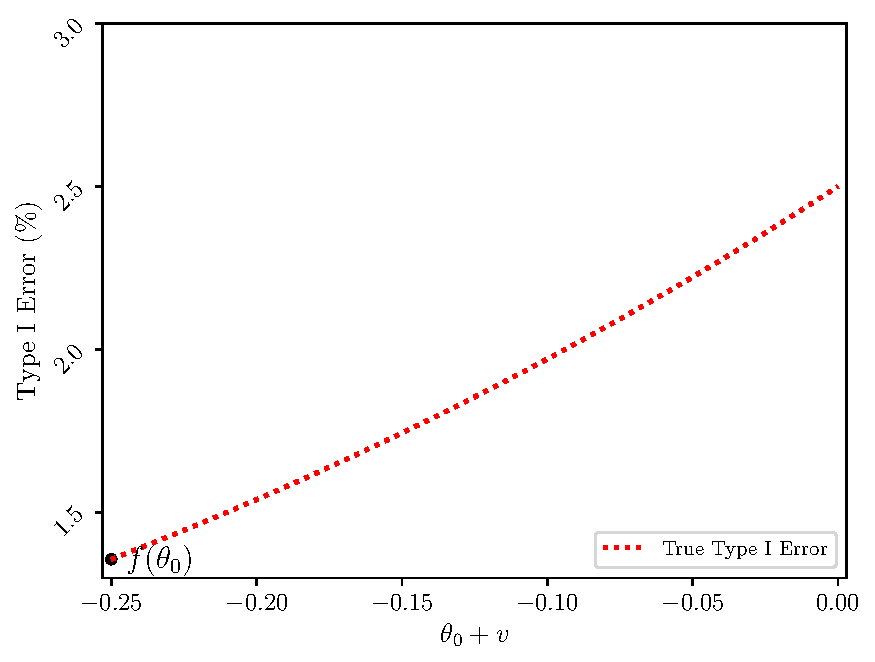
\includegraphics[width=0.85\linewidth]{figs/greens_up_tie.pdf}
\end{figure}
\begin{itemize}
    \item $X \sim \normal\pr{\theta, 1}$, $\Theta = [-0.25, 0]$.
    \item $\design(X)$: reject if $X > z_{1-\alpha}$.
\end{itemize}
\end{frame}

\begin{frame}{The Tilt-Bound for a Particular $q$}
\begin{figure}
    \centering
    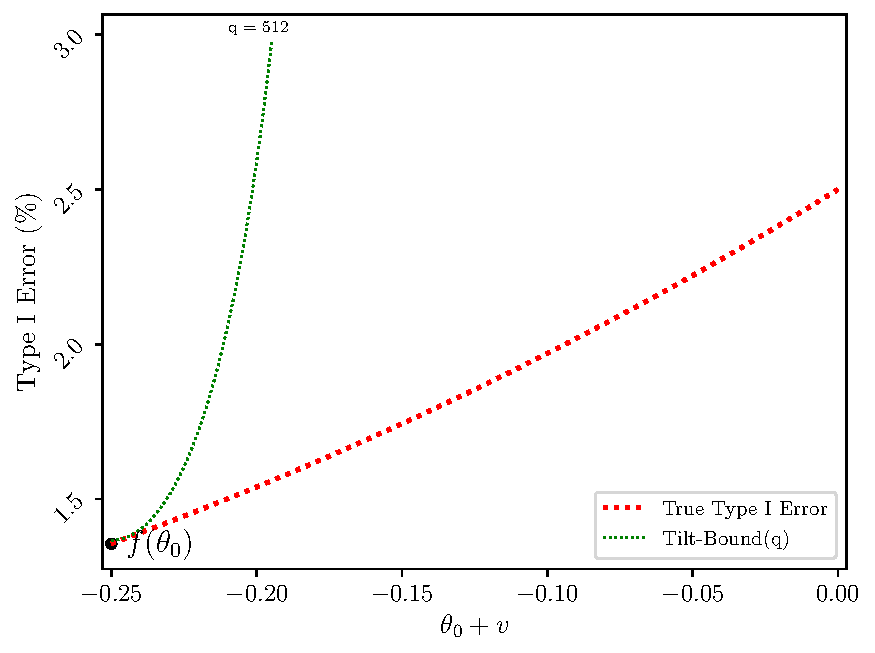
\includegraphics[width=0.85\linewidth]{figs/greens_up_one_q.pdf}
\end{figure} 
\begin{equation*}
    U(\theta_0, v, q, f(\theta_0))
    =
    f(\theta_0)^{1 - \frac{1}{q}} 
    \exp\sbr{\frac{(q - 1) v^2}{2}}
\end{equation*}
\end{frame}

\begin{frame}{The Tilt-Bound for Many $q$s}
\begin{figure}
    \centering
    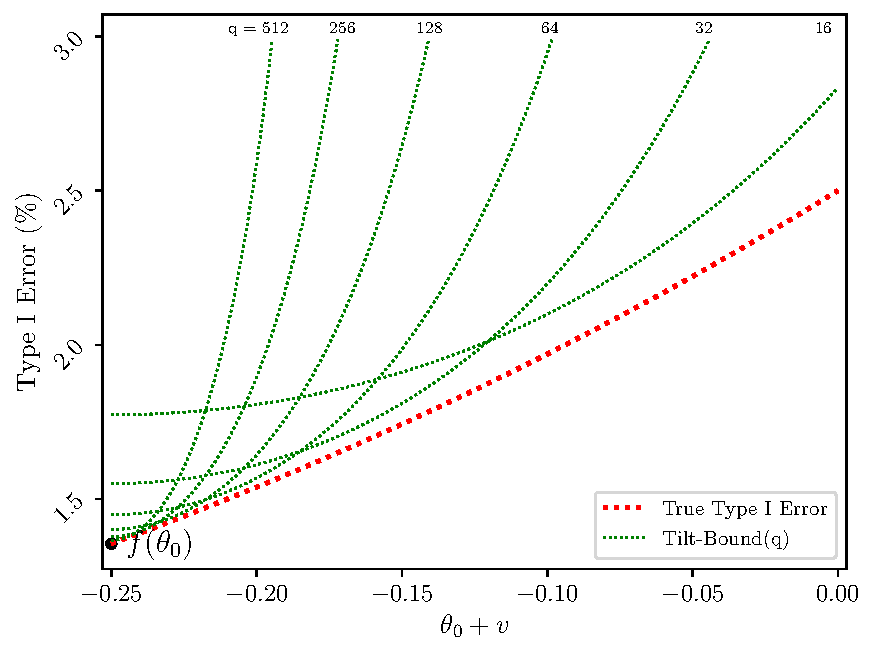
\includegraphics[width=0.85\linewidth]{figs/greens_up_all_q.pdf}
\end{figure} 
\begin{equation*}
    U(\theta_0, v, q, f(\theta_0))
    =
    f(\theta_0)^{1 - \frac{1}{q}} 
    \exp\sbr{\frac{(q - 1) v^2}{2}}
\end{equation*}
\end{frame}

\begin{frame}{The Optimized Tilt-Bound is Tight}
\begin{figure}
    \centering
    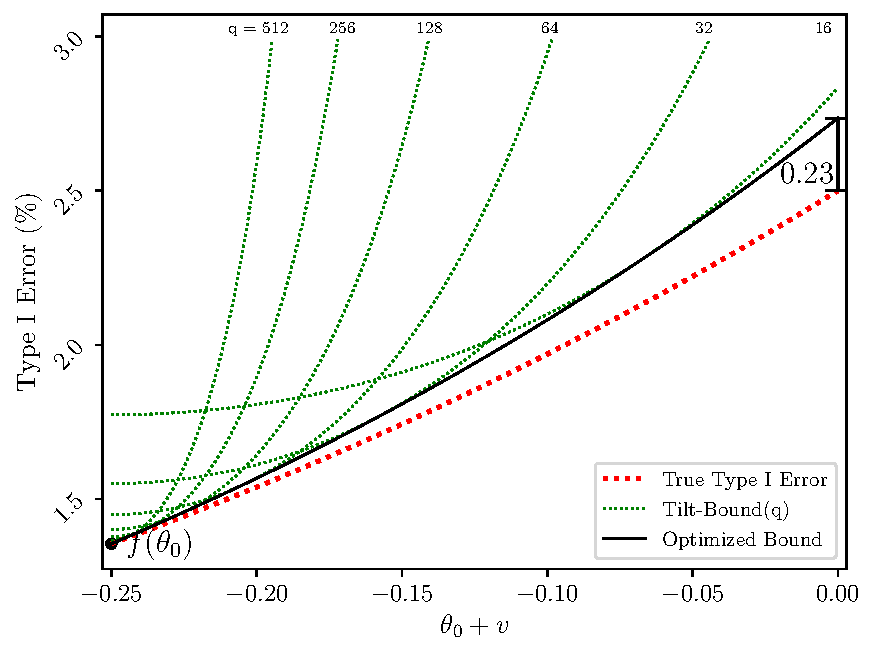
\includegraphics[width=0.85\linewidth]{figs/greens_up.pdf}
\end{figure} 
\begin{equation*}
 \inf\limits_{q \geq 1} U(\theta_0, v, q, f(\theta_0))
\end{equation*}
\end{frame}

\begin{frame}{Tilt-Bound Summary}
\begin{itemize}
    \item Tilt-Bound is a \textbf{deterministic} bound.
    \item Tight over small to medium distances.
    \item Valid for \textbf{any rejection set}.
    \item Depends on Type I Error at the 
    \textbf{initial point $\theta_0$} and 
    the \textbf{distributional family $P_\theta$} 
    (which implicitly accounts for the sample size).
\end{itemize}
\end{frame}
\subsection{Validation}
\frame{\tableofcontents[currentsubsection]}

\begin{frame}{Main Task: Point-wise Valid Upper Bound on Type I Error}
\begin{figure}
    \centering
    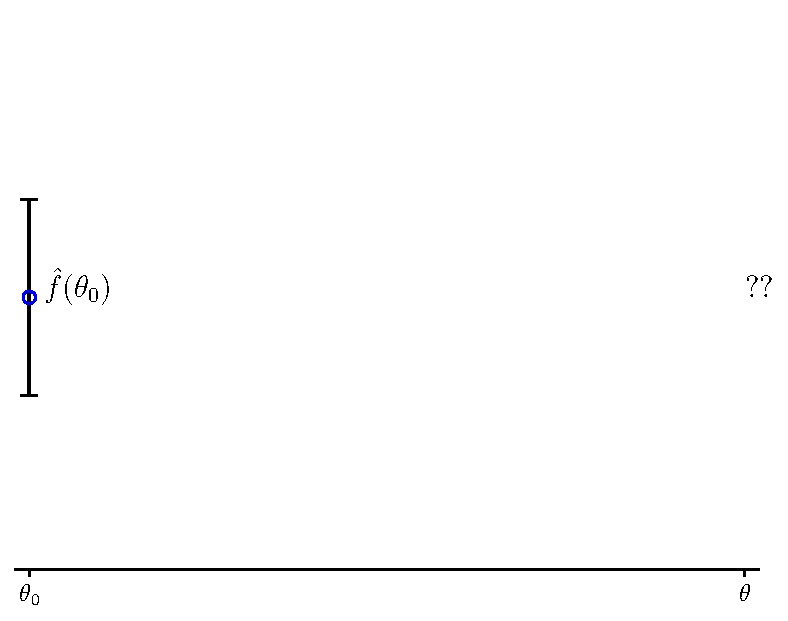
\includegraphics[width=0.75\linewidth]{figs/validation_problem.pdf}
\end{figure}
\begin{itemize}
    \item $X \sim P_\theta$ (known distribution), null space $\Theta$.
    \item Any arbitrary design $\design$.
    \item Clopper-Pearson bound using Monte Carlo estimate $\hat{f}(\theta_0)$.
\end{itemize} 
\end{frame}

\begin{frame}{Claim: Valid Upper Bound on the Type I Error}
\begin{figure}
    \centering
    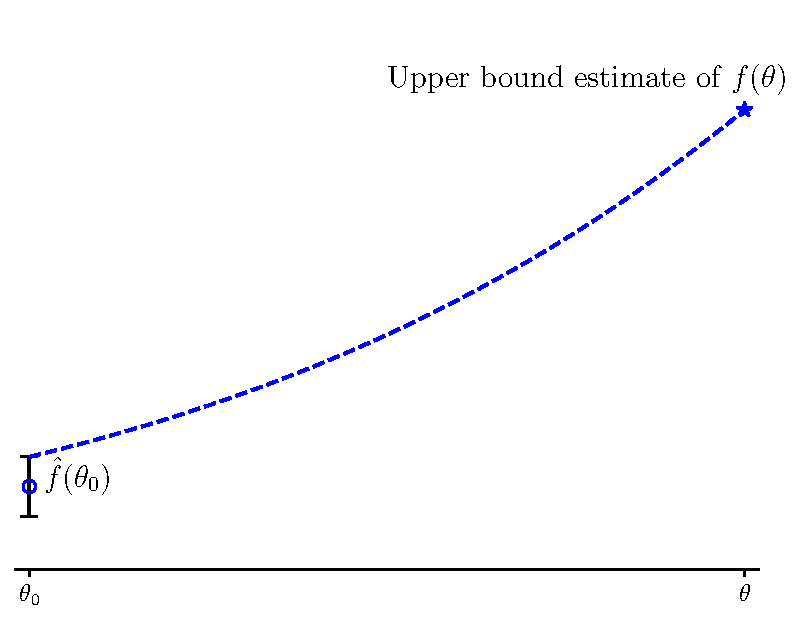
\includegraphics[width=0.95\linewidth]{figs/validation_solution.pdf}
\end{figure} 
\end{frame}

\begin{frame}{Use Tilt-Bound on Upper Bound Estimate!}
\textbf{Monotone Property:}
\begin{itemize}
    \item $a \mapsto U(\theta_0, v, q, a)$ is \textbf{non-decreasing}.
\end{itemize}

\textbf{Validation Proof:} 
\begin{itemize}
    \item $\hat{\eta}$ be a $1-\delta$ upper bound of $f(\theta_0)$.
    \item $\hat{u} := U(\theta_0, v, q, \hat{\eta})$ for any $q \geq 1$.
\end{itemize}
Recall,
\begin{align*}
    f(\theta_0 + v)
    \leq
    U(\theta_0, v, q, f(\theta_0))
\end{align*}
Then,
\begin{align*}
    \prob\pr{f(\theta_0+v) \leq \hat{u}}
    \geq
    \prob\pr{f(\theta_0) \leq \hat{\eta}}
    \geq
    1-\delta
\end{align*}
\end{frame}

\begin{frame}{Use Tilt-Bound on a Grid for the Z-Test}
\begin{figure}
    \centering
    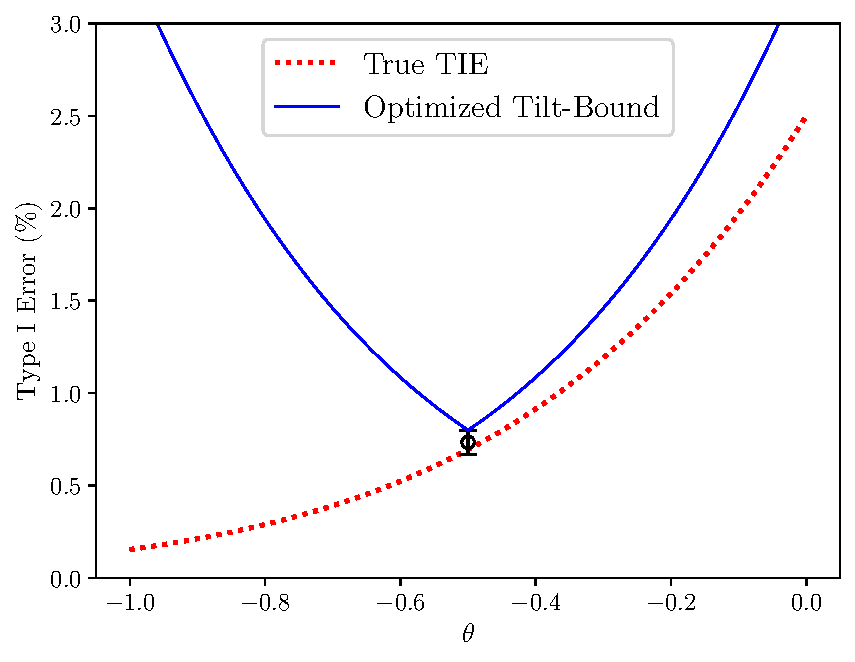
\includegraphics[width=0.95\linewidth]{figs/validation_1.pdf}
\end{figure} 
\end{frame}

\begin{frame}{Use Tilt-Bound on a Grid for the Z-Test}
\begin{figure}
    \centering
    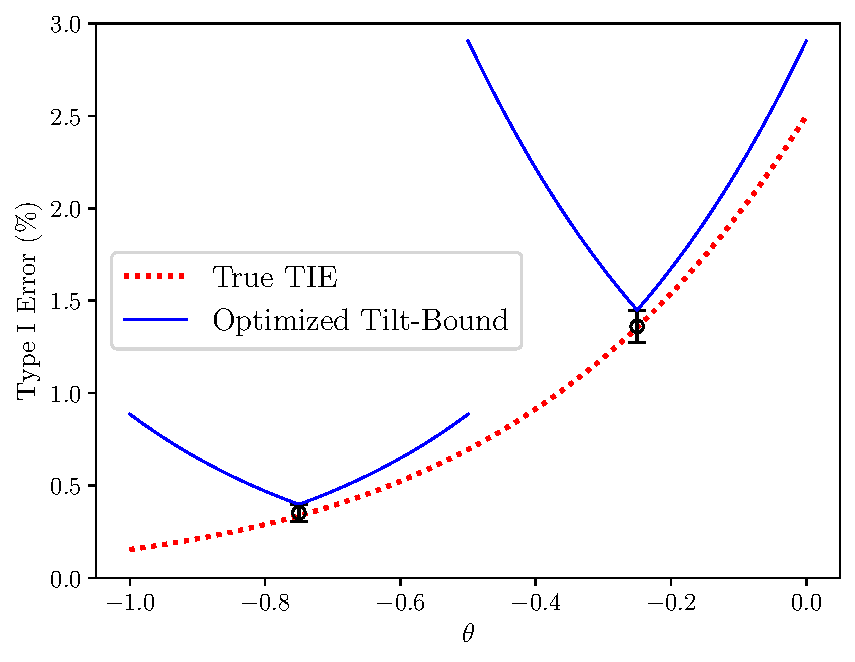
\includegraphics[width=0.95\linewidth]{figs/validation_2.pdf}
\end{figure} 
\end{frame}

\begin{frame}{Use Tilt-Bound on a Grid for the Z-Test}
\begin{figure}
    \centering
    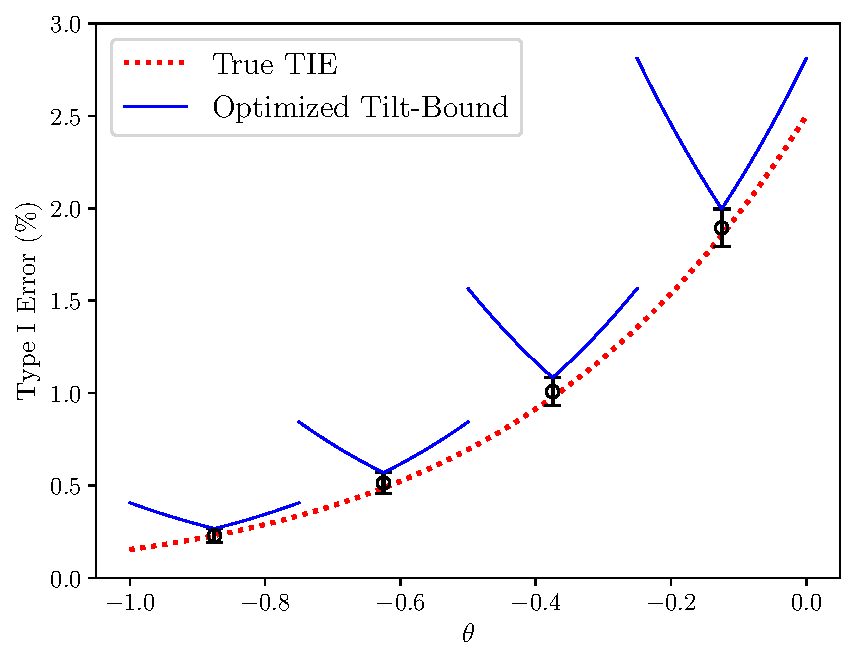
\includegraphics[width=0.95\linewidth]{figs/validation_4.pdf}
\end{figure} 
\end{frame}

\begin{frame}{Use Tilt-Bound on a Grid for the Z-Test}
\begin{figure}
    \centering
    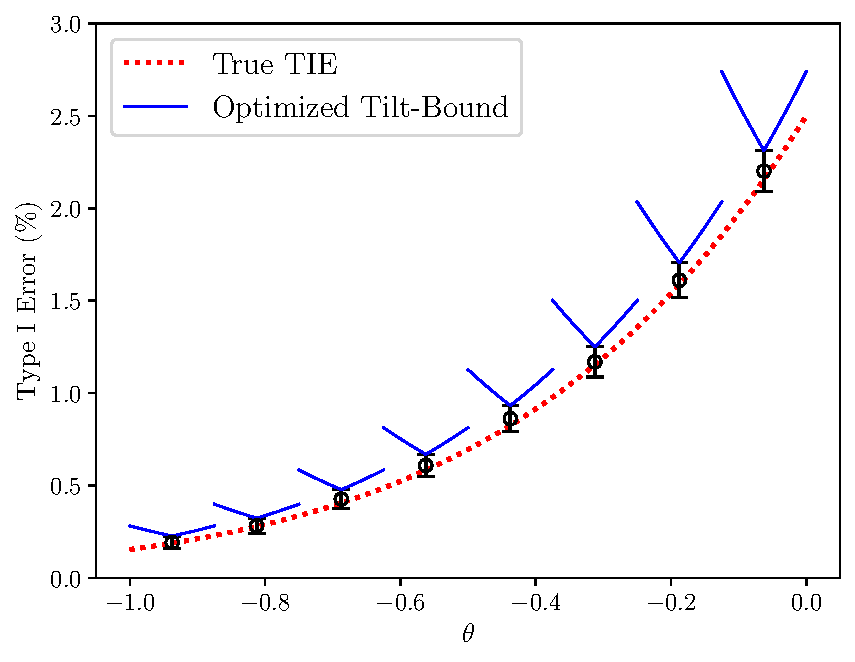
\includegraphics[width=0.95\linewidth]{figs/validation_8.pdf}
\end{figure} 
\end{frame}

\begin{frame}{Use Tilt-Bound on a Grid for the Z-Test}
\begin{figure}
    \centering
    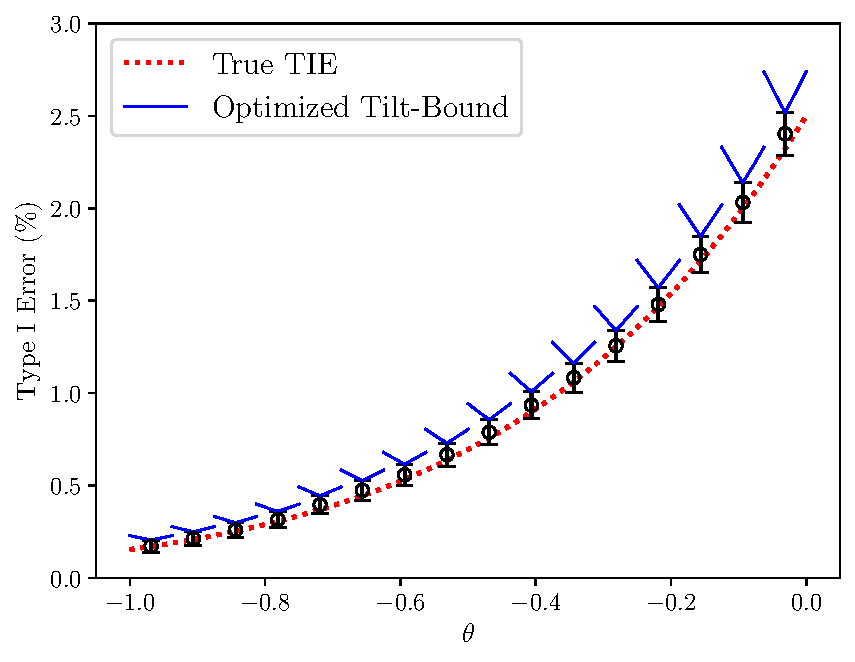
\includegraphics[width=0.95\linewidth]{figs/validation_16.pdf}
\end{figure} 
\end{frame}

\begin{frame}{Use Tilt-Bound on a Grid for the Z-Test}
\begin{figure}
    \centering
    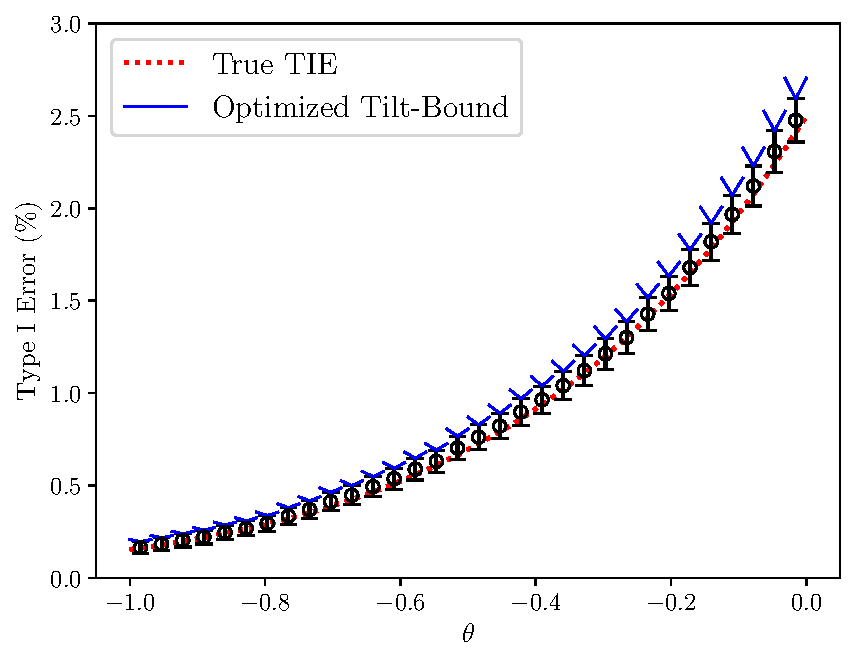
\includegraphics[width=0.95\linewidth]{figs/validation_32.pdf}
\end{figure} 
\end{frame}

\begin{frame}{Use Tilt-Bound on a Grid for the Z-Test}
\begin{figure}
    \centering
    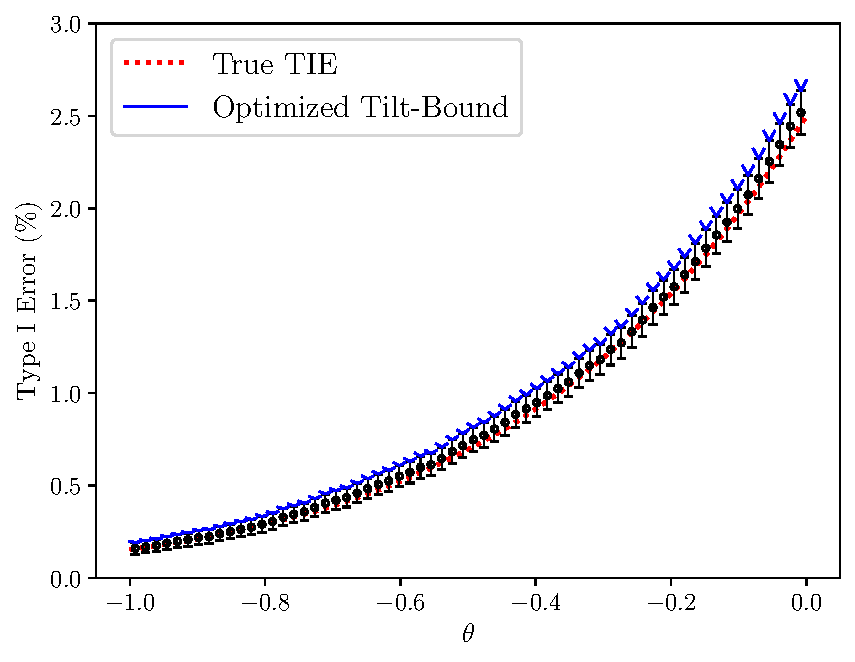
\includegraphics[width=0.95\linewidth]{figs/validation_64.pdf}
\end{figure} 
\end{frame}
\subsection{Calibration}
\frame{\tableofcontents[currentsubsection]}

\begin{frame}{Main Task: Find Critical Threshold with Level $\alpha$ at $\theta_0$}
\begin{figure}
    \centering
    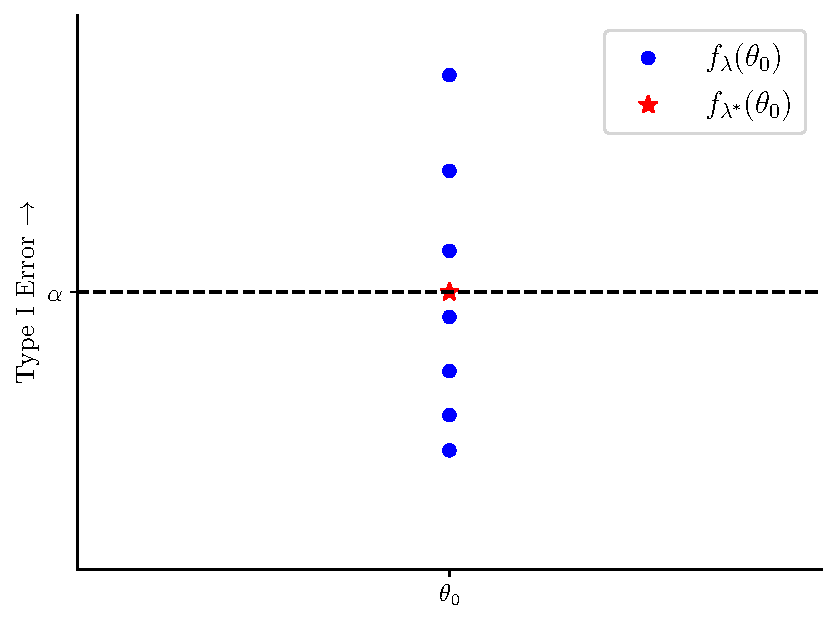
\includegraphics[width=0.95\linewidth]{figs/calibration_point_null.pdf}
\end{figure} 
\end{frame}

\begin{frame}{Straightforward for a Single Point}
\begin{itemize}
    \item Let $S(X)$ be the test statistic with data $X$.
    \item Design $\design$: rejects if $S(X) < \lambda$.
    \item Given $S_1,\ldots, S_N$ i.i.d. test statistics,
        \begin{align*}
            \hat{\lambda}^* := S_{\floor{(N+1) \alpha}}
            \implies
            \EEE\br{f_{\hat{\lambda}^*}(\theta_0)} \leq \alpha
        \end{align*}
    \item Easy to show using Beta distribution.
\end{itemize} 
\end{frame}

\begin{frame}{Calibration Results for a Single Point}
\begin{figure}
    \centering
    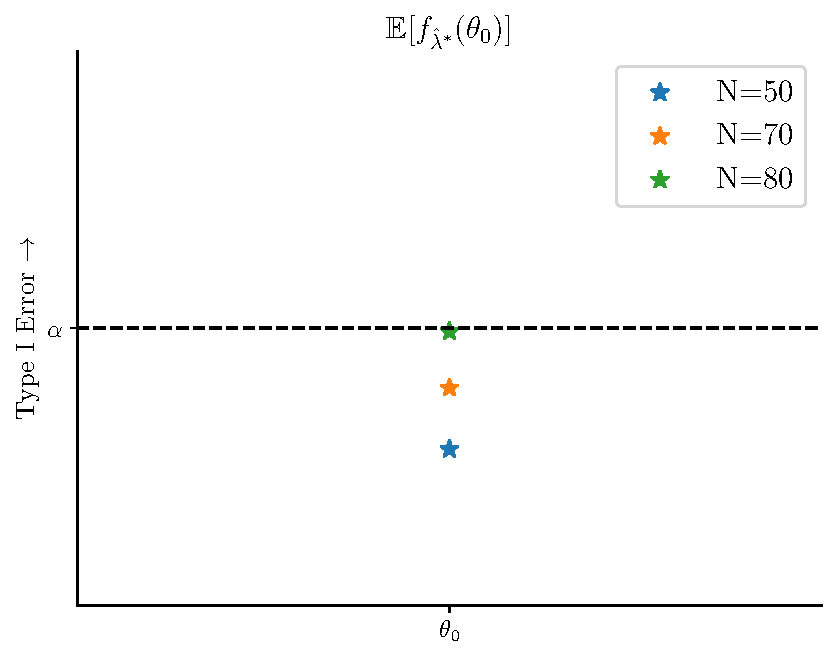
\includegraphics[width=0.9\linewidth]{figs/calibration_point_null_solution.pdf}
\end{figure} 
\end{frame}

\begin{frame}{Main Task: Find Critical Threshold with Level $\alpha$ at $\theta$}
 \begin{figure}
     \centering
     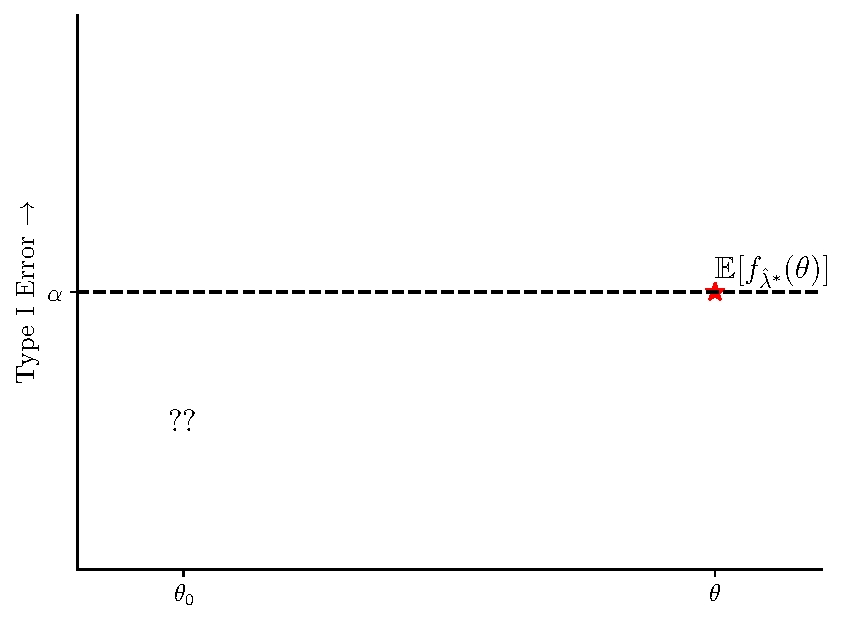
\includegraphics[width=0.95\linewidth]{figs/calibration_tile.pdf}
 \end{figure}
\end{frame}

\begin{frame}{Inverted Tilt-Bound}
Claim: Calibrate at $\theta_0$ to Control Tilt-Bound at $\theta$
\begin{figure}
    \centering
    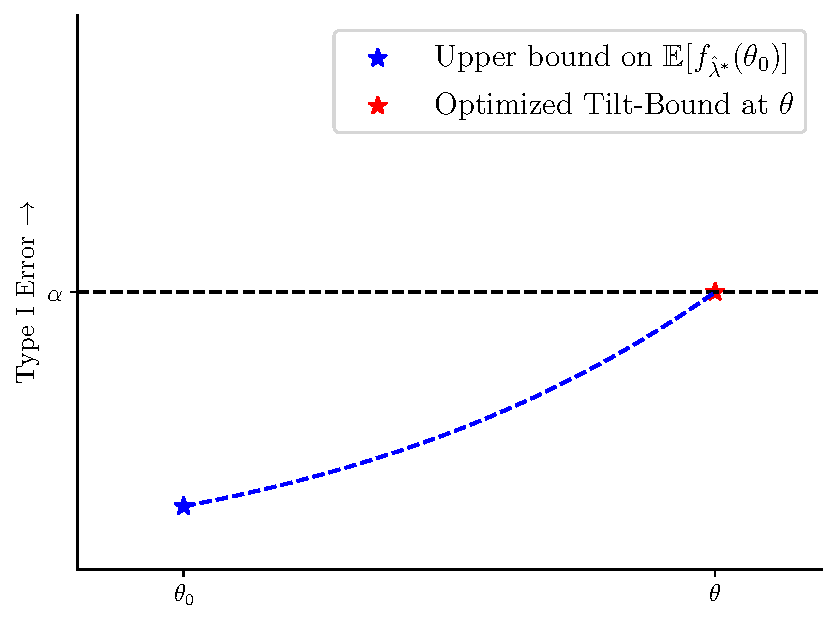
\includegraphics[width=0.9\linewidth]{figs/calibration_tile_solution.pdf}
\end{figure} 
\end{frame}

%\begin{frame}{Extending point-null case to a tile using CSE}
%\begin{itemize}
%    \item Assume $\Theta$ a region around a point $\theta_0$.
%    \item Back-solve from the worst-case Tilt-bound over $\Theta$ (which always occurs at a corner of $\Theta$).
%    \item Find a level $\alpha' < \alpha$ so that
%    \begin{equation}
%        \EEE\br{f_{\lambda}(\theta_0)} \leq \alpha' 
%        \implies
%        \sup \limits_{\theta \in \Theta}
%        \EEE\br{f_{\lambda}(\theta)} \leq \alpha
%    \end{equation}
%    \item Then it suffices to point-calibrate at $\theta_0$ with target level $\alpha'$.
%\end{itemize} 
%\end{frame}

\begin{frame}{Use CSE to Control Type I Error at $\theta$}
\begin{align*}
    \EEE\br{f_{\lambda}(\theta_0+v)}
    &\leq
    U(\theta_0, v, q, \EEE\br{f_{\lambda}(\theta_0)})
\end{align*} 
\begin{itemize}
    \item Back-solve to hit level $\alpha$:
        \begin{align*}
            U(\theta_0, v, q, \EEE\br{f_{\lambda}(\theta_0)})
            \leq 
            \alpha
            \iff
            \EEE\br{f_\lambda(\theta_0)}
            \leq 
            U^{-1}(\theta_0, v, q, \alpha)
        \end{align*}
\end{itemize} 
\textbf{Inverted Tilt-Bound:}
\begin{equation*}
    U^{-1}(\theta_0, v, q, \alpha) 
    := \pr{
    \alpha \exp\br{
    -\frac{\psi(\theta_0, v, q)}{q} 
    + \psi(\theta_0, v, 1)
    }}^{\frac{q}{q-1}}
\end{equation*}
\end{frame}

\begin{frame}{Use Point-Null Case to Find Critical Threshold}
\begin{itemize}
    \item Let $\alpha' := U^{-1}(\theta_0, v, q, \alpha)$.
    \item Find $\hat{\lambda}^*$ such that
        \begin{align*}
            \EEE\br{f_{\hat{\lambda}^*}(\theta_0)} \leq \alpha'
        \end{align*}
    \item Maximize $\alpha'$ over $q \geq 1$ 
        for free to get least-conservative threshold.
\end{itemize} 
Then,
\begin{align*}
    \EEE\br{f_{\hat{\lambda}^*}(\theta_0 + v)}
    \leq
    U(\theta_0, v, q, \EEE\br{f_{\hat{\lambda}^*}(\theta_0)})
    \leq
    \alpha
\end{align*}
\end{frame}

\begin{frame}{Control Type I Error in a Region}
\begin{itemize}
    \item Back-solve with \textbf{worst-case} Tilt-Bound:
        \begin{align*}
            &\sup\limits_{v \in \Theta-\theta_0}
            U(\theta_0, v, q, \EEE\br{f_{\lambda}(\theta_0)})
            \leq 
            \alpha
            \\\iff \quad
            &\EEE\br{f_\lambda(\theta_0)}
            \leq 
            \inf\limits_{v \in \Theta-\theta_0}
            U^{-1}(\theta_0, v, q, \alpha)
        \end{align*}
    \item Let $\alpha' := \inf\limits_{v \in \Theta -\theta_0} U^{-1}(\theta_0, v, q, \alpha)$.
    \item Maximize $\alpha'$ over $q \geq 1$.
    \item Find $\hat{\lambda}^*$ such that 
        \begin{align*}
            \EEE\br{f_{\hat{\lambda}^*}(\theta_0)} \leq \alpha'
        \end{align*}
\end{itemize} 
\end{frame}

\begin{frame}{How to optimize over $v$?}
\begin{align*}
    \inf\limits_{v \in \Theta-\theta_0}
    U^{-1}(\theta_0, v, q, \alpha)
\end{align*} 
\begin{itemize}
    \item \textbf{Assume a linearity condition}!
    \item Inverted Tilt-Bound is \textbf{quasi-concave} in $v$, respectively!
    \item If $\Theta$ is a polytope, suffices to compute only at the vertices!
\end{itemize} 
\end{frame}

\begin{frame}{How to optimize over $v$?}
\begin{theorem}[Quasi-convex in $v$]
Let $\set{P_{\theta} : \theta \in \Theta \subseteq \R^d}$ be a family of distributions:
\begin{align*}
    dP_{\theta}(x) = \exp\sbr{g_{\theta}(x) - A(\theta)} d\mu(x)
\end{align*}
Fix any $\theta_0 \in \Theta$.
Suppose that $\Delta(v, x) \equiv g_{\theta_0+v}(x) - g_{\theta_0}(x)$ 
is linear in $v$, i.e.
$\Delta(v, x) = W(x)^\top v$ 
for some $W(x) \in \R^d$.
Then, the Inverted Tilt-Bound is quasi-concave as a function of $v$.
\end{theorem}
\end{frame}

\begin{frame}{Divide-and-Conquer yields a Global Guarantee}
\begin{itemize}
    \item Assume $\Theta$ any bounded space.
    \item Partition $\Theta$ into tiles $\set{\Theta_i}_{i=1}^I$ 
        with representatives $\set{\theta_i}_{i=1}^I$.
    \item Calibrate to get $\hat{\lambda}^*_i$ for each tile $\Theta_i$.
    \item Take the most conservative, $\hat{\lambda}^* := \min\limits_{i=1,\ldots, I} \hat{\lambda}^*_i$.
    \item Then,
        \begin{align*}
            \sup\limits_{\theta \in \Theta}
            \EEE\br{f_{\hat{\lambda}^*}(\theta)}
            &=
            \max\limits_{i=1,\ldots,I}
            \sup\limits_{\theta \in \Theta_i}
            \EEE\br{f_{\hat{\lambda}^*}(\theta)}
            \\&\leq 
            \max\limits_{i=1,\ldots,I}
            \sup\limits_{\theta \in \Theta_i}
            \EEE\br{f_{\hat{\lambda}^*_i}(\theta)}
            \\&\leq
            \alpha
        \end{align*}
\end{itemize} 
\end{frame}

\begin{frame}{Type I Error Tightens with More Simulations and Tiles}
\begin{figure}
    \centering
    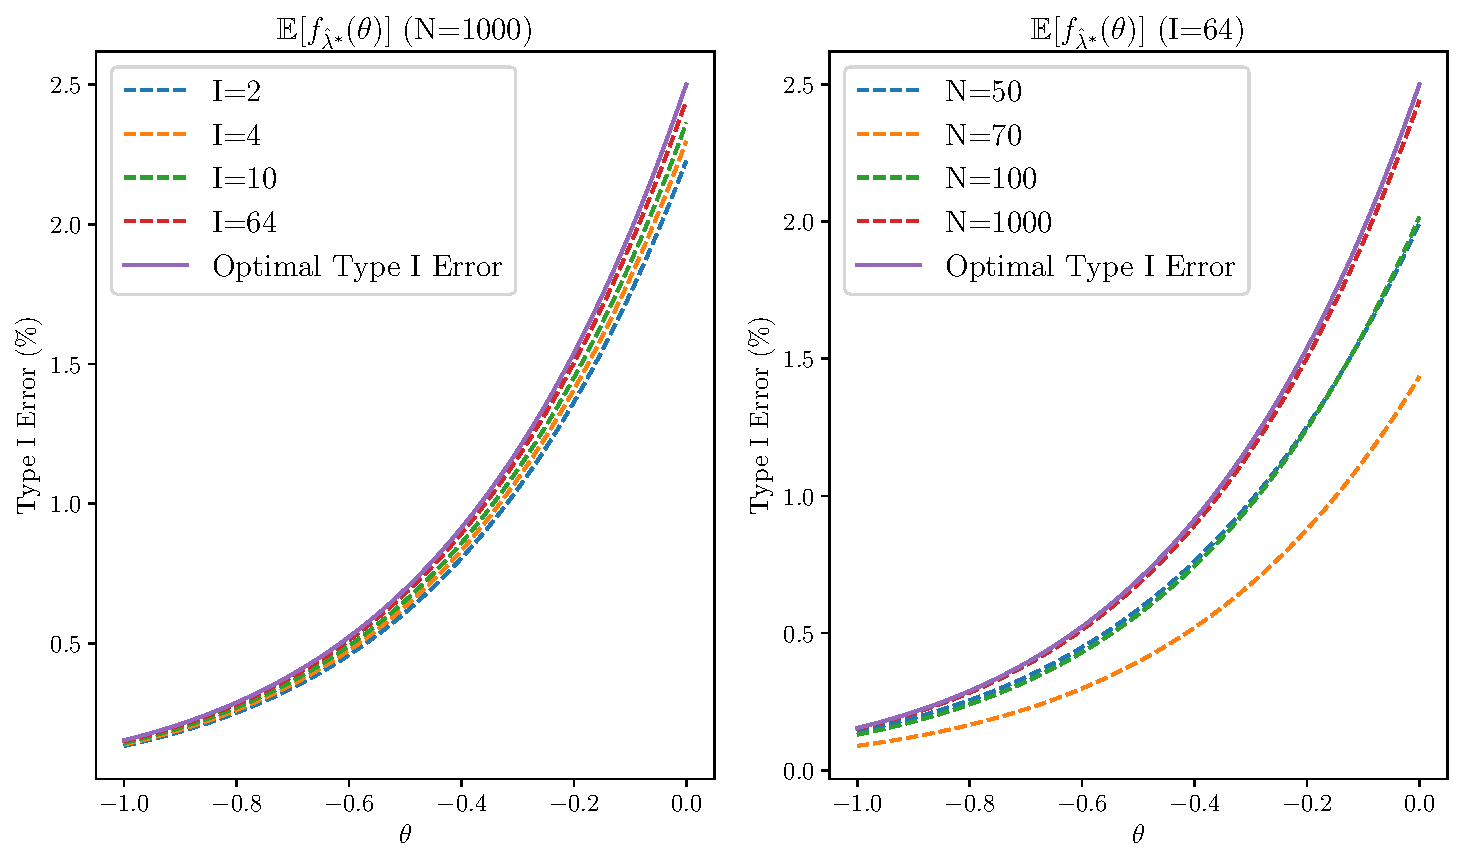
\includegraphics[width=\linewidth]{figs/calibration_z_test.pdf}
\end{figure} 
\end{frame}



\subsection{Adaptive T-Test}
\frame{\tableofcontents[currentsubsection]}

\begin{frame}{Revisiting the Adaptive T-Test}
\begin{itemize}
    \item Data $X_i \sim \normal\pr{\mu, \sigma^2}$
        with unknown $\mu, \sigma^2$.
    \item $H_0: \mu \leq \mu_0$.
    \item Initial sample size of $n_0$.
    \item $K$ interims where each interim stops 
        if the t-statistic given observed data up to now
        is above the threshold $t^*$.
    \item If continue, add $n_i$ more data.
    \item Final analysis: reject if t-statistic is above $t^*$.
\end{itemize} 
\begin{align*}
    \theta_0 := \frac{\mu}{\sigma^2}
    \quad
    \theta_1 := -\frac{1}{2\sigma^2}
\end{align*}
\end{frame}

\begin{frame}{Tight Analysis Despite Lack of Exact Theory}
\begin{figure}
    \centering
    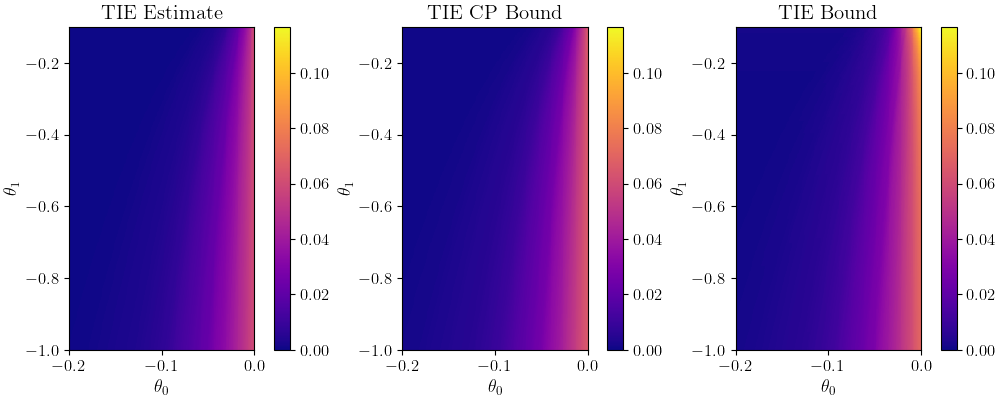
\includegraphics[width=\linewidth]{figs/t_test_adaptive.png}
\end{figure} 
\end{frame}

\begin{frame}{Adaptive T-Test Computation and Configuration}
\begin{itemize}
    \item \textbf{Computation:}
    \begin{itemize}
        \item 327 million simulations.
        \item Runtime: 2s.
        \item M1 Macbook Pro.
    \end{itemize}
    \item \textbf{Configuration:}
    \begin{itemize}
        \item $K=3$ interims.
        \item $n_0 = 100$.
        \item $n_i = 50$ for $1 \leq i \leq K$.
        \item $\mu_0 = 0$.
        \item $\alpha = 0.025$.
    \end{itemize}
\end{itemize}
\end{frame}

\subsection{Bayesian Basket Trial}

\begin{frame}{Bayesian Basket Trial from~\citet{berry:2013}}
\begin{itemize}
    \item Design:
        \begin{align*}
            Y_j &\sim \Binom(n_j, p_j) \quad j=1,\ldots, d \\
            \theta_j &= \theta_{0j} + \logit(p_j) \\
            \theta_j &\sim \normal\pr{\mu, \sigma^2} \\
            \mu &\sim \normal\pr{\mu_0, \sigma_0^2} \\
            \sigma^2 &\sim \Gamma^{-1}\pr{\alpha_0, \beta_0}
        \end{align*}
    \item Let $c \in \br{0,1}^{d-1}$ be a vector of fixed thresholds and $d \equiv 4$.
    \item Reject if $\prob\br{p_i > p_0 | Y} > c_i$ for some null (treatment) arm $i$.
\end{itemize}
\end{frame}

\begin{frame}{Validation shows Type I Error Surface for Bayesian Design}
\begin{figure}
    \centering
    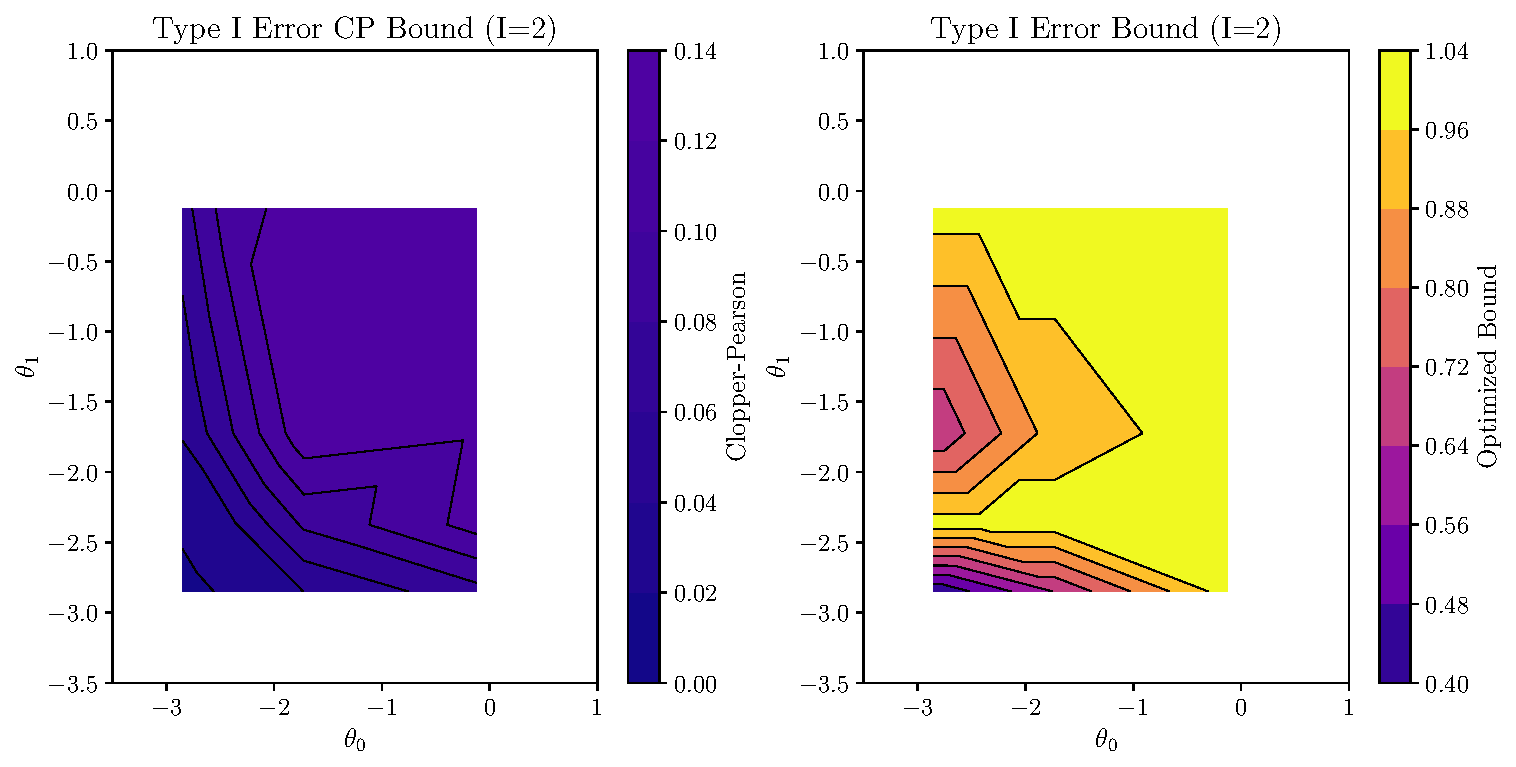
\includegraphics[width=\linewidth]{figs/berry_0.pdf}
\end{figure}
\end{frame}

\begin{frame}{Validation shows Type I Error Surface for Bayesian Design}
\begin{figure}
    \centering
    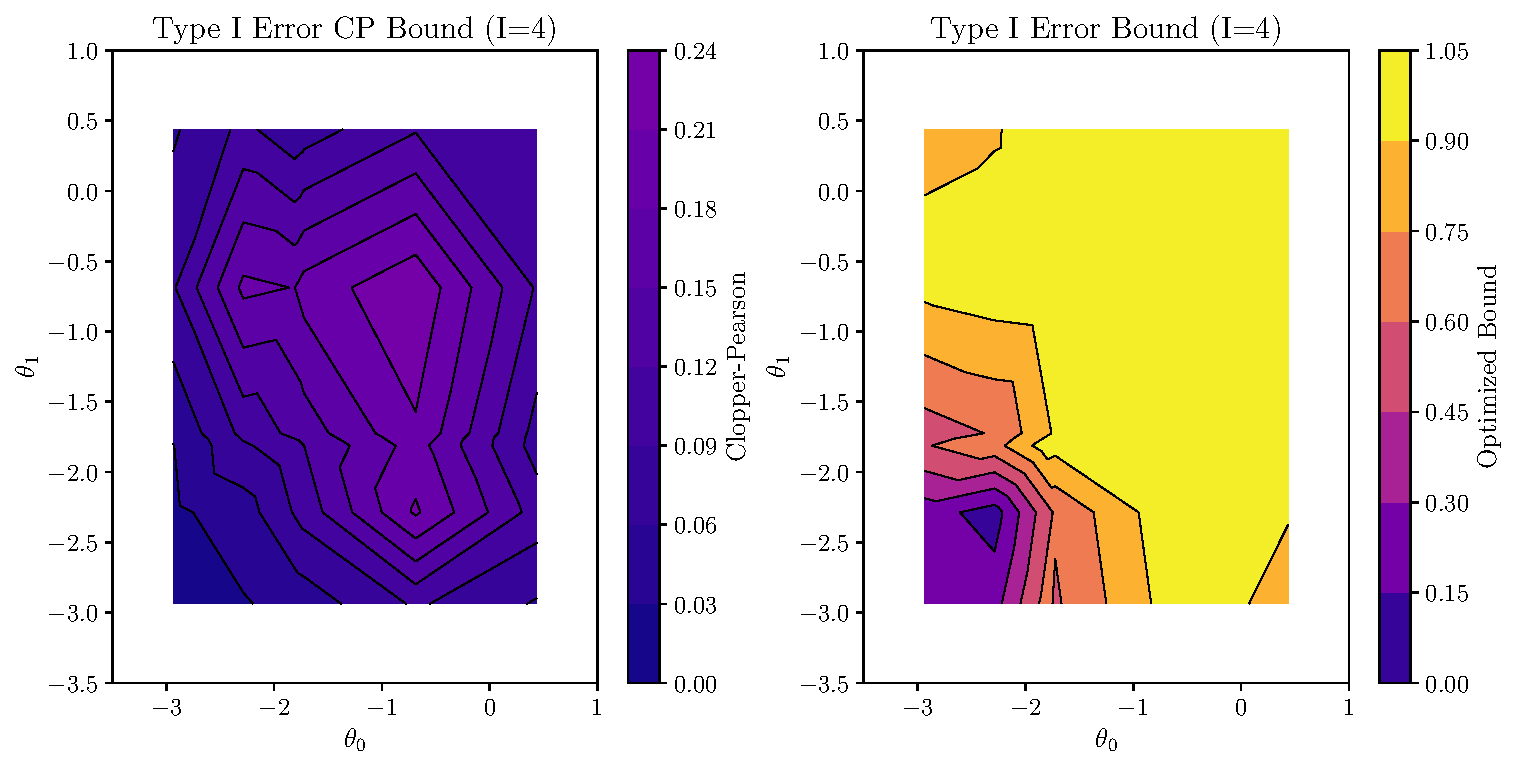
\includegraphics[width=\linewidth]{figs/berry_1.pdf}
\end{figure}
\end{frame}

\begin{frame}{Validation shows Type I Error Surface for Bayesian Design}
\begin{figure}
    \centering
    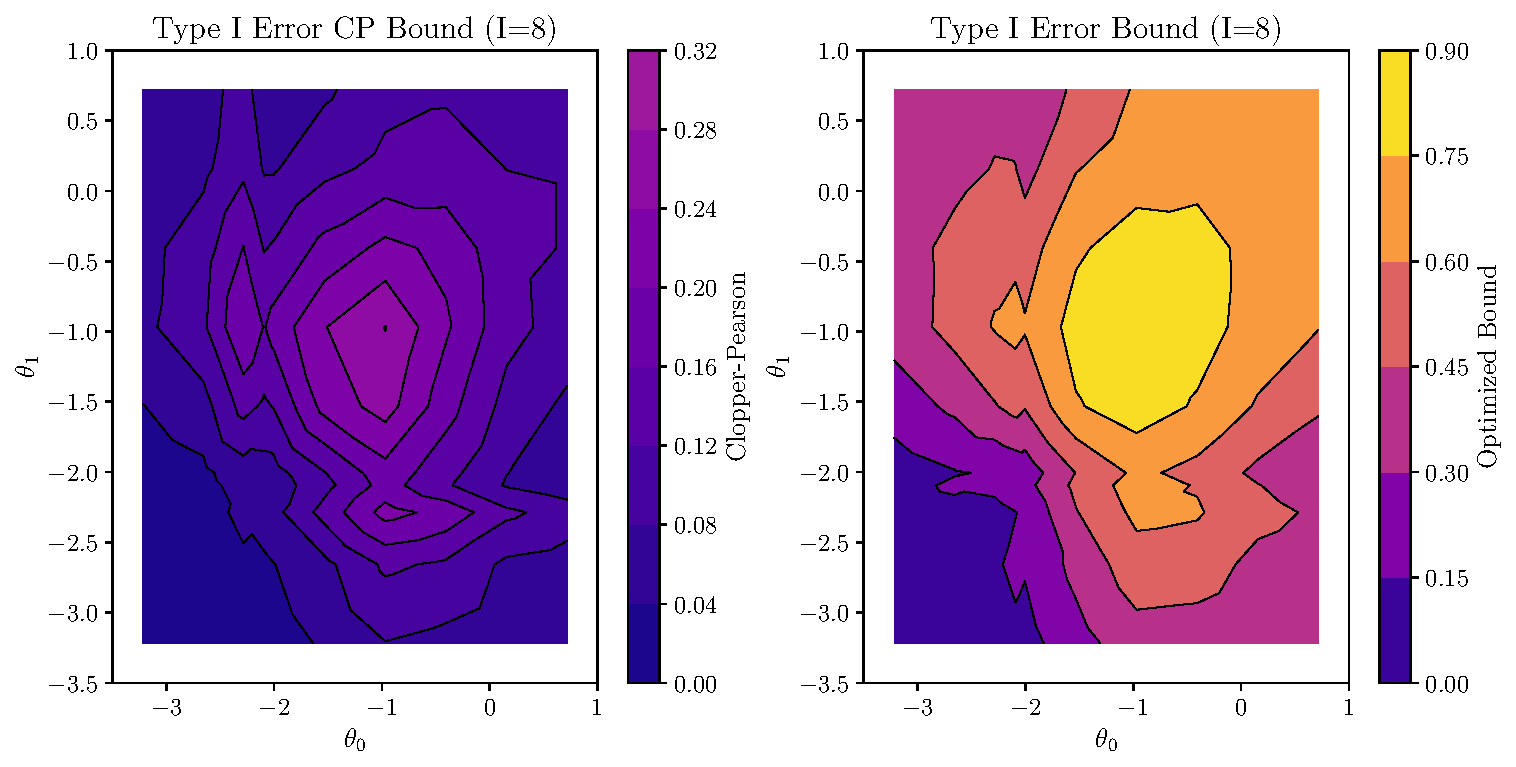
\includegraphics[width=\linewidth]{figs/berry_2.pdf}
\end{figure}
\end{frame}

\begin{frame}{Validation shows Type I Error Surface for Bayesian Design}
\begin{figure}
    \centering
    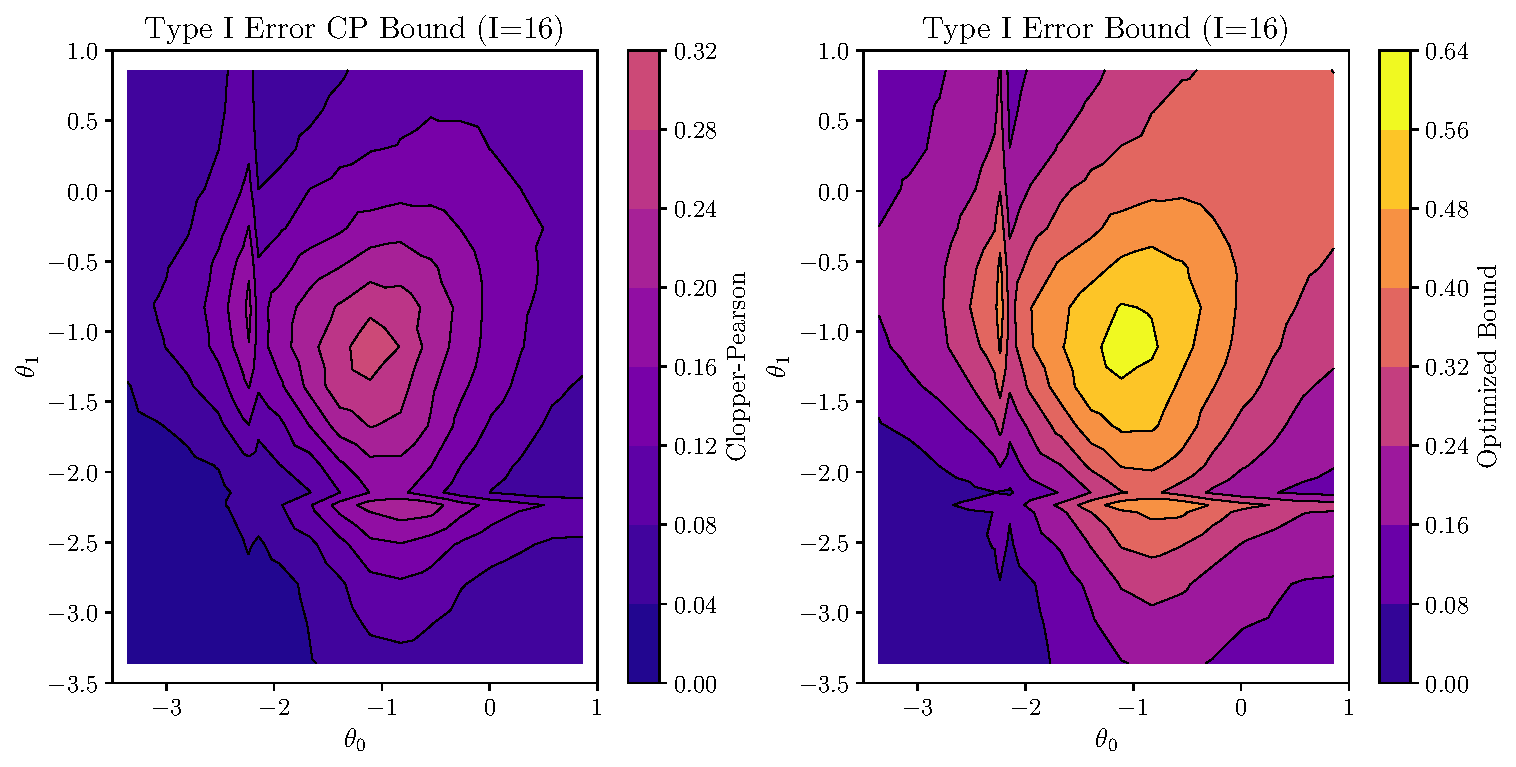
\includegraphics[width=\linewidth]{figs/berry_3.pdf}
\end{figure}
\end{frame}

\begin{frame}{Validation shows Type I Error Surface for Bayesian Design}
\begin{figure}
    \centering
    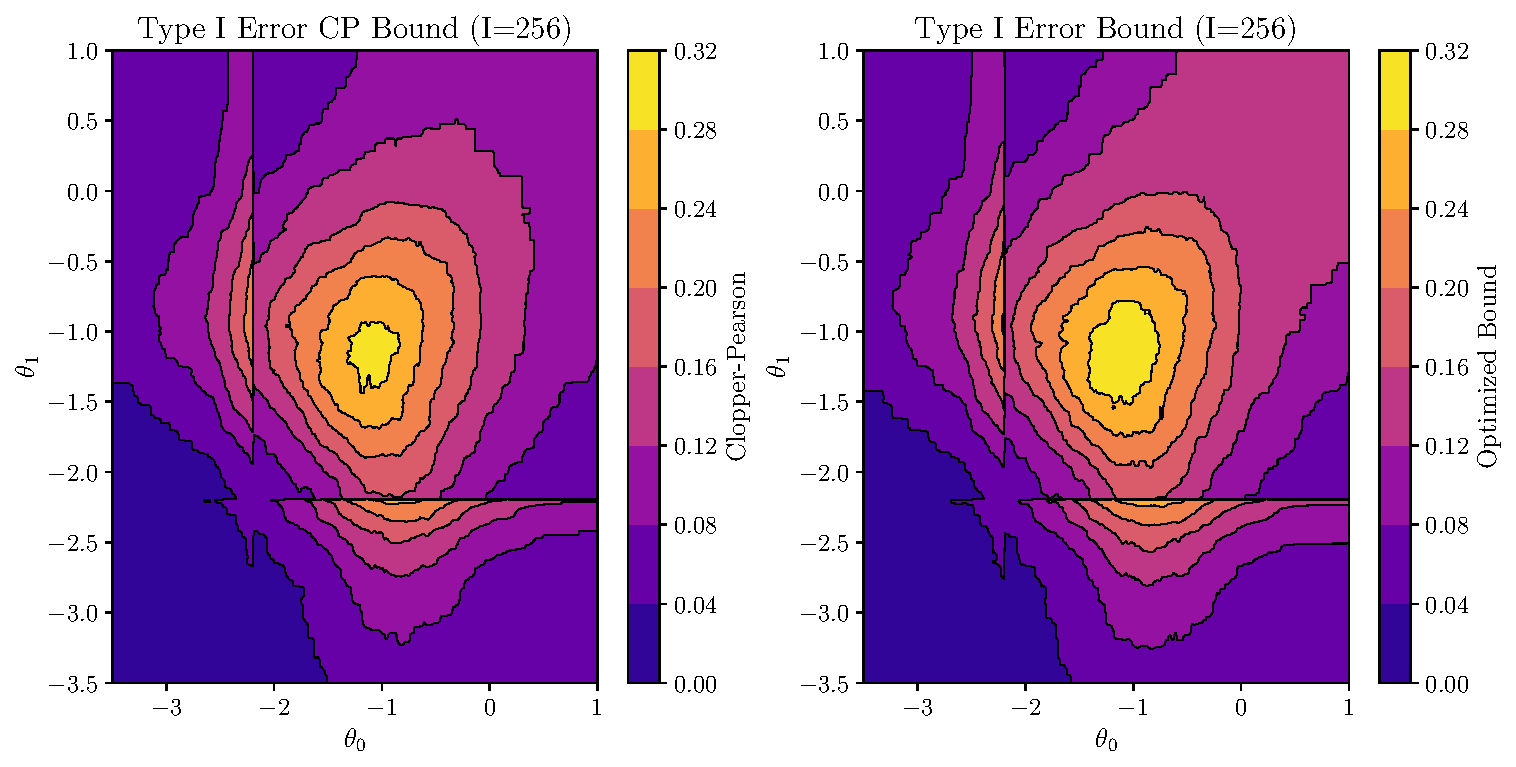
\includegraphics[width=\linewidth]{figs/berry_4.pdf}
\end{figure}
\end{frame}

\begin{frame}{\citet{berry:2013} Computation and Configuration}
\begin{itemize}
    \item \textbf{Computation}:
    \begin{itemize}
        \item 7.34 trillion simulations.
        \item Runtime: 4 hours.
        \item Nvidia V100 GPU.
    \end{itemize}
    \item \textbf{Configuration:}
    \begin{itemize}
        \item $n_i = 35$ for all $i=1,\ldots, d$.
        \item $\mu_0=-1.34$, $\sigma_0 = 10$, $\alpha_0 = 0.0005$, 
            $\beta_0 = 0.000005$.
        \item $c_i = 0.85$ for all $i=1,\ldots, d$.
    \end{itemize}
\end{itemize} 
\end{frame}

%\begin{frame}{\citet{berry:2013} Remarks (Optional)}
%\begin{itemize}
%    \item Type I Error is high in some areas! 
%    \item Type I Error is well-controlled at global null: $\theta_i = \theta_{0i}$.
%    \item This is unsurprising, because ~\citet{berry:2013} had calibrated this design for control only at the global null.
%\end{itemize}
%\end{frame}

\subsection{Complex Phase II/III Selection Design}

\begin{frame}{A Complicated Phase II/III Selection Design}
\begin{itemize}
    \item 3 treatment and 1 control arm with binary outcomes.
    \item Trial decisions using the Bayesian hierarchical model 
        as in~\citet{berry:2013}.
    \item Stage 1: select the ``best'' treatment arm against control
        with interim analyses.
    \item Each of 3 interim analyses can stop for futility,
    drop one or more poorly performing treatments,
    or accelerate an arm to move to stage 2.
    \item Stage 2: one interim and one final analysis. 
    \item The total number of patients across
        all arms and stages is at most 800 with at most 350 in any single arm.
\end{itemize} 
\end{frame}

\begin{frame}{Phase II/III Selection Design Calibrated Successfully}
\begin{figure}
    \centering
    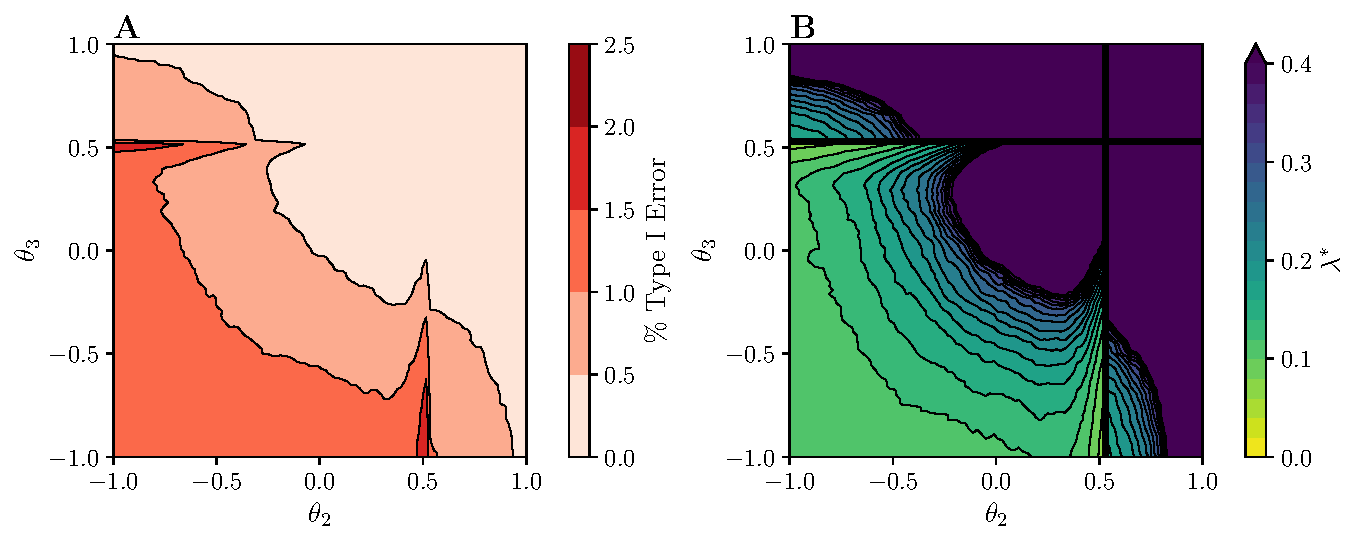
\includegraphics[width=\linewidth]{figs/lewis_tie_lam.pdf}
    \caption{%
    Both plots slice the domain by fixing 2 parameters, $\theta_0 = \theta_1 = 0.533$. Figure \textbf{A} shows the Tilt-Bound profile for the selected threshold $\hat{\lambda}^* = 0.06253$. Figure \textbf{B} shows the critical value $\hat{\lambda}^*_i$ separately for each tile such that its Tilt-Bound is 2.5\%.}
\end{figure} 
\end{frame}

\begin{frame}{Phase II/III Selection Design Computation and Configuration}
\begin{itemize}
    \item \textbf{Computation:}
    \begin{itemize}
        \item 960 billion simulations.
        \item Runtime: 5 days.
        \item Nvidia V100 GPU.
    \end{itemize}
    \item \textbf{Configuration:}
    \begin{itemize}
        \item $H_0: \theta_i \leq \theta_0$ for all $i=1,\ldots, d-1$.
        \item Restrict to $\theta_i \in [-1,1]$ for all $i$.
    \end{itemize}
\end{itemize}
\end{frame}

\begin{frame}{Phase II/III Selection Design Remarks (Optional)}
\begin{itemize}
    \item Max Tilt-Bound occurs at the tile with center
        $\theta_0 = (0.4925, 0.4925, 0.4925, -1.0)$. 
    \item Paradox: worst Type I Error \textbf{does not} 
        occur at the global null (where all treatments perform equally to control), but when \textbf{one} treatment performs poorly.
\end{itemize} 
\end{frame}
\section{Conclusion}
\frame{\tableofcontents[currentsection]}

\begin{frame}{Further Results of CSE}
\begin{itemize}
    \item Can study \textbf{power, False Discovery Rate (FDR)}, and \textbf{bias of bounded estimators}.
    \item Theory also holds for \textbf{Generalized Linear Models (GLMs)} after conditioning on covariates.
    \begin{itemize}
        \item E.g. logistic regression.
    \end{itemize}
    \item \textbf{Quasi-convexity} results for the Tilt-Bound/Inverted Tilt-Bound simplify computations to checking vertices.
    \item See pre-print for details.
\end{itemize} 
\end{frame}

\begin{frame}{Computational Tricks}
    \begin{itemize}

    \item Adaptive simulation/grid sizing (dramatic overall cost reduction!).

    \item Correlated simulations (dramatic sampling reduction!). 
    \begin{itemize}
        \item \textbf{BoTorch} uses a similar (more advanced) trick.
        \item Thanks to \textbf{Prof. Art Owen} for the idea!
    \end{itemize}
    
    \item How to perform \textbf{1 trillion simulations} of a complex Bayesian design? 
    \begin{itemize}
        \item \textbf{Integrated Nested Laplace Approximation (INLA)}.
        \item Our INLA code is \textbf{1 million times faster} than standard MCMC packages.
        \item Similar accuracy in most cases.
    \end{itemize}

    \end{itemize}
\end{frame}

\begin{frame}{Remarks}
\begin{itemize}
    \item Proof-by-simulation is \textbf{general, powerful, and robust}.
    \item Continuous Simulation Extension converts
        simulations at finite points
        into guarantees over \textbf{regions}.

    \item Practical advantage: CSE analyzes the design 
        \textbf{as represented in code}. Robust to:
        \begin{itemize}
            \item Approximations.
            \item Theoretical uncertainties with convergence of algorithms
        \end{itemize}
    \item With the right software, method is \textbf{tractable}!
\end{itemize} 
\end{frame}

\begin{frame}{End Goals}
%\begin{itemize}
%    \item We hope these tools can streamline innovation in trial design
%    \item Objective proofs should help improve regulatory consistency
%    \item Reducing the time and human capital cost of validating new procedures is good for everyone
%    \item Speculatively: this might pave the way to use ``black-box" statistical procedures. Our guarantees would apply, as long as the model class assumption is trusted.
%\end{itemize}
\begin{itemize}
    \item Streamline innovation in trial design.
    \item Improve regulatory consistency with objective proofs.
    \item Reduce time and human capital cost of validating new procedures.
    \item Speculatively: enable new ``black-box" statistical procedures.
\end{itemize}
\end{frame}


\begin{frame}[allowframebreaks]
\frametitle{References}
\bibliographystyle{plainnat}
\bibliography{references}
\end{frame}

%\begin{frame}{Normal Inverted Tilt-Bound}
%\begin{figure}
%    \centering
%    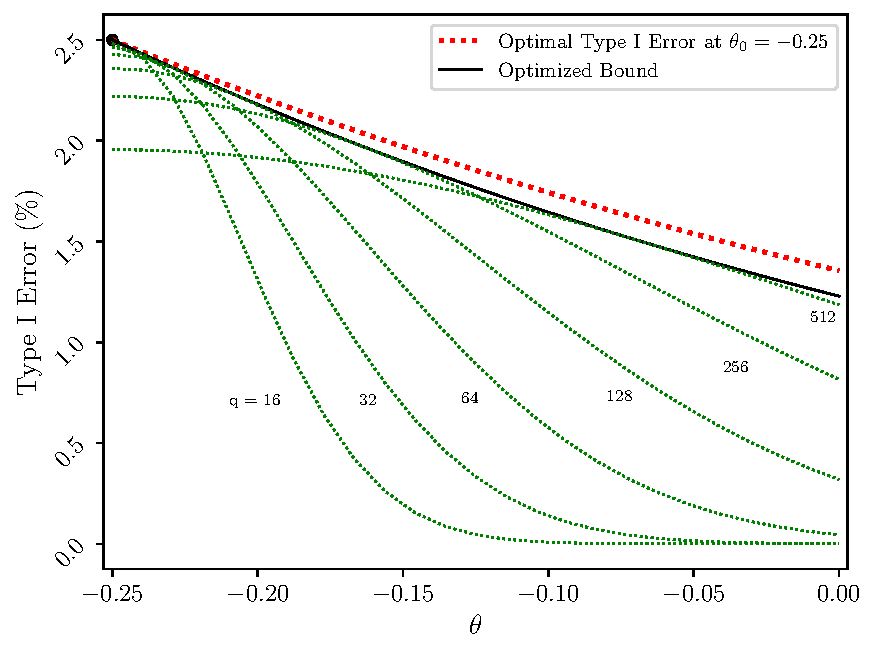
\includegraphics[width=0.8\linewidth]{figs/greens_down.pdf}
%\end{figure} 
%\begin{equation*}
%    U^{-1}(\theta_0, v, q, \alpha)
%    =
%    \pr{
%    \alpha \exp\br{-\frac{(q-1) v^2}{2}}
%    }^{\frac{q}{q-1}}
%\end{equation*}
%\end{frame}


\end{document}
